\documentclass{IEEEtran}
\usepackage[T1]{fontenc}
\usepackage[utf8]{inputenc}
\usepackage[brazil]{babel}
\usepackage{graphicx}
\usepackage{amsmath}
\usepackage{amssymb}
\usepackage{cite}
\usepackage{booktabs}
\usepackage{hyperref}
\usepackage{url}
\usepackage{natbib}
\usepackage{enumitem}
\usepackage{array}
\usepackage{multirow}
\usepackage{xcolor}
\usepackage[table]{xcolor}
\usepackage{array}
\usepackage{booktabs}
\usepackage{multirow}
\usepackage{graphicx} % para \resizebox
\usepackage{listings}
\usepackage[utf8]{inputenc}   % (não necessário em LaTeX moderno / lualatex/xelatex)
\usepackage{xcolor}
\usepackage{booktabs}
\usepackage{multirow}
\usepackage{array}

\markboth{}{PLN -- UFSCar 2026: Projeto de Processamento de Linguagem Natural}

\title{Sentimento como Relevância: Recomendação de Produtos em E-commerce Brasileiro}

\author{%
  Cilene Renata Real$^{1}$,
  Jayme Sakae dos Reis Furuyama$^{1}$,
  Wesley Nogueira Galvão 3$^{1}$,
  $^{1}$Programa de Pós-Graduação em Ciência da Computação (PPGCC),
  Universidade Federal de São Carlos (UFSCar), São Carlos, SP, Brasil\\
  \texttt{\{real.cilene, jaymefuryama\}@gmail.com}\\
  \texttt{wesleygalvao@estudante.ufscar.br}
}

\begin{document}
\maketitle

% =========================================================
\begin{abstract}
A análise de sentimentos em avaliações de produtos é uma das tarefas mais estudadas em Processamento de Linguagem Natural (PLN), com forte aplicabilidade em plataformas de e-commerce. Este trabalho propõe um sistema integrado de duas etapas: (i)~um classificador de polaridade de sentimento (positivo/negativo) a ser treinado sobre avaliações em português brasileiro do corpus B2W-Reviews01, comparando representações baseadas em TF-IDF e \textit{embeddings} contextuais do BERTimbau; e (ii)~um motor de recomendação de produtos que recuperará itens semanticamente similares pelo título, re-ranqueando os resultados por um \textit{score} de positividade derivado do modelo com melhor desempenho. Os classificadores serão avaliados com precisão, revocação, F1-macro e AUC-ROC, e o módulo de recomendação com NDCG@k e Precision@k, complementados por avaliação qualitativa conduzida pelos integrantes do grupo. Espera-se que a combinação de representações densas com análise de sentimento agregue valor significativo à qualidade das recomendações em domínios ruidosos de texto gerado por usuário.
\end{abstract}

% =========================================================
\section{Introdução}
\label{sec:intro}

Plataformas de comércio eletrônico acumulam diariamente volumes massivos de avaliações escritas por consumidores. Essas avaliações constituem uma fonte rica de opinião sobre produtos, entrega e experiência de compra, porém permanecem majoritariamente subutilizadas nos sistemas de recomendação tradicionais, que tendem a depender exclusivamente de dados de interação (cliques, compras e notas numéricas) \cite{ahmed2025sentimentaware}.

Análise de sentimentos (AS) é a tarefa de PLN que visa inferir automaticamente a polaridade afetiva de um texto partir de seu conteúdo \cite{alzahrani2022intelligent}. O seu objetivo é estudar e extrair opiniões, avaliações, atitudes, apreciações e emoções direcionadas a entidades como produtos, serviços, indivíduos, tópicos ou eventos \cite{BPLN_livro_4ed:2026}. A análise pode ser conduzida em três níveis de granularidade: no nível do documento (avaliando a polaridade geral do texto), no nível da sentença, ou no nível do aspecto

Quando aplicada a avaliações de produtos, ela permite mapear opiniões para um sinal de qualidade que complementa a nota numérica fornecida pelo consumidor. O corpus B2W-Reviews01 \cite{real2019b2w}, formado por mais de 130 mil avaliações da Americanas.com em português brasileiro, é um recurso público representativo desse domínio, com anotações de nota (1--5 estrelas), recomendação binária e metadados demográficos dos avaliadores.

Dois desafios fundamentais motivam este projeto. O primeiro é a representação adequada do texto em português para tarefas de classificação: abordagens baseadas em vetorização esparsa oferecem uma linha de base eficiente e interpretável \cite{BPLN_livro_4ed:2026}, enquanto modelos de vetorização densa capturam dependências semânticas e contextuais que as superam em diversas tarefas \cite{jm3}. O segundo desafio é a integração do sinal de sentimento em um motor de recomendação: recuperar produtos similares pelo título por meio de busca vetorial e re-ranquear os resultados pelo índice de positividade das avaliações classifica melhor os itens que os consumidores efetivamente recomendam.

Desta forma, o presente projeto propõe um \textit{pipeline} completo que: (a) realiza análise exploratória e pré-processamento do corpus B2W-Reviews01; (b) compara dois paradigmas de representação textual para classificação de sentimento binária; (c) constrói um banco vetorial dos títulos de produtos; e (d) entrega recomendações re-ranqueadas pelo sentimento. O sistema final é avaliado tanto quantitativamente quanto por análise qualitativa conduzida pelos integrantes do grupo.

O restante do relatório está organizado da seguinte forma: a Seção~\ref{sec:related} apresenta os trabalhos relacionados; a Seção~\ref{sec:methodology} descreve a metodologia detalhada; A Seção ~\ref{sec:discussion} discute os resultados apresentados e suas comparações entre os modelos; e a Seção~\ref{sec:conclusion} traz as considerações finais e os próximos passos.

% =========================================================
\section{Trabalhos Relacionados}
\label{sec:related}

\subsection{Análise de Sentimentos em Avaliações de E-commerce}

% A análise de sentimentos em avaliações de produtos é uma área amplamente estudada. \citeauthor{alzahrani2022intelligent}~\cite{alzahrani2022intelligent} propuseram um sistema baseado em aprendizado profundo combinando CNN, LSTM e BERT para classificar avaliações de e-commerce em múltiplas polaridades, obtendo acurácia superior a 94\% em conjuntos de dados em inglês. Os autores destacam que avaliações são ruidosas -- com erros tipográficos, gírias e linguagem informal -- e que o pré-processamento adequado é fundamental para o desempenho dos modelos.
%  Ajeitando a citação
A análise de sentimentos em avaliações de produtos é uma área amplamente estudada. Alzahrani \textit{et al.}~\cite{alzahrani2022intelligent} propuseram um sistema baseado em aprendizado profundo combinando CNN, LSTM e BERT para classificar avaliações de e-commerce em múltiplas polaridades, obtendo acurácia superior a 94\% em conjuntos de dados em inglês. Os autores destacam que avaliações são ruidosas, com erros tipográficos, gírias e linguagem informal, e que o pré-processamento adequado é fundamental para o desempenho dos modelos.

% Para o português brasileiro, a situação é mais desafiadora pela escassez de recursos anotados. \citeauthor{souza2022bert}~\cite{souza2022bert} realizaram um estudo comparativo sistemático entre TF-IDF com Regressão Logística (linha de base), embeddings do BERTimbau (pré-treinado sem ajuste fino) e BERTimbau com \textit{fine-tuning} em datasets de sentimento em português. Os autores demonstraram que o BERTimbau com \textit{fine-tuning} supera consistentemente a linha de base TF-IDF, atingindo AUC-ROC superior a 0.95 em múltiplos benchmarks, e que a versão \textit{large} do modelo apresenta ganhos marginais em relação à versão \textit{base}.

%  Ajeitando a citação
Para o português brasileiro, a situação é mais desafiadora pela escassez de recursos anotados. Sousa e Filho\cite{souza2022bert} realizaram um estudo comparativo sistemático entre TF-IDF com Regressão Logística (linha de base), embeddings do BERTimbau (pré-treinado sem ajuste fino) e BERTimbau com \textit{fine-tuning} em datasets de sentimento em português. Os autores demonstraram que o BERTimbau com \textit{fine-tuning} supera consistentemente a linha de base TF-IDF, atingindo AUC-ROC superior a 0.95 em múltiplos benchmarks, e que a versão \textit{large} do modelo apresenta ganhos marginais em relação à versão \textit{base}.


\subsection{Modelos de Linguagem Pré-treinados: BERT e BERTimbau}

O BERT (\textit{Bidirectional Encoder Representations from Transformers}) \cite{devlin2019bert} revolucionou o PLN ao propor o pré-treinamento bidirecional profundo sobre grandes corpora, seguido de \textit{fine-tuning} supervisionado para tarefas específicas. Diferente de modelos anteriores, o BERT condiciona simultaneamente os contextos esquerdo e direito em todas as suas camadas de atenção, produzindo representações contextuais ricas.

O BERTimbau \cite{souza2020bertimbau} é a adaptação do BERT para o português brasileiro, pré-treinado no corpus BrWaC (\textit{Brazilian Web as Corpus}) com aproximadamente 2,7 bilhões de palavras. O modelo está disponível nas versões \textit{base} (110M parâmetros) e \textit{large} (335M parâmetros) e estabeleceu novos estados da arte em reconhecimento de entidades nomeadas, similaridade textual e implicação textual em português.

\subsection{TF-IDF como Representação para Classificação de Texto}

A ponderação TF-IDF (\textit{Term Frequency--Inverse Document Frequency}) \cite{manning2008introduction} é uma das representações esparsas mais utilizadas em tarefas de classificação de texto. Combinada com classificadores lineares como a Regressão Logística, essa abordagem serve como linha de base interpretável e de baixo custo computacional. Por não capturar dependências contextuais, o TF-IDF com Regressão Logística pode, em certos cenários, apresentar desempenho competitivo frente a modelos mais complexos, especialmente em domínios com vocabulário especializado e textos curtos \cite{souza2022bert}.

\subsection{Recomendação de Produtos Orientada por Sentimento}
% Ajeitando citação
% A integração de análise de sentimentos em sistemas de recomendação tem crescido significativamente. \citeauthor{vaishnavi2023sentiment}~\cite{vaishnavi2023sentiment} propuseram um sistema que combina classificação de sentimento das avaliações com XGBoost e CatBoost e usa a saída para construir matrizes de similaridade item-item baseadas em similaridade de cosseno, reportando melhorias no RMSE frente a sistemas baseados apenas em notas numéricas. 

A integração de análise de sentimentos em sistemas de recomendação tem crescido significativamente. Vaishnavi e Kalpana~\cite{vaishnavi2023sentiment} propuseram um sistema que combina e classifica o sentimento das avaliações com XGBoost e CatBoost e usa a saída para construir matrizes de similaridade item-item baseadas em similaridade de cosseno, reportando melhorias no RMSE frente a sistemas baseados apenas em notas numéricas.


Uma revisão abrangente recente \cite{ahmed2025sentimentaware} categoriza os sistemas de recomendação orientados por sentimento em quatro grandes abordagens: (i) classificadores de aprendizado profundo que combinam embeddings de sentimento com interações usuário-item; (ii) métodos baseados em Transformers para extração de features; (iii) redes neurais em grafos que propagam sinais de sentimento; e (iv) recomendadores conversacionais que se adaptam em tempo real ao \textit{feedback} do usuário. O trabalho de Darraz \textit{et al.}~\cite{sharma2025enhancing} demonstrou que incorporar sentimento via BERT em filtragem colaborativa reduz o RMSE para 1,2478 em benchmarks do Yelp, reforçando a relevância da abordagem proposta neste projeto.

% Ajeitando citação
% Uma revisão abrangente recente \cite{ahmed2025sentimentaware} categoriza os sistemas de recomendação orientados por sentimento em quatro grandes abordagens: (i) classificadores de aprendizado profundo que combinam embeddings de sentimento com interações usuário-item; (ii) métodos baseados em Transformers para extração de features nuançadas; (iii) redes neurais em grafos que propagam sinais de sentimento; e (iv) recomendadores conversacionais que se adaptam em tempo real ao \textit{feedback} do usuário. O trabalho de \citeauthor{sharma2025enhancing}~\cite{sharma2025enhancing} demonstrou que incorporar sentimento via BERT em filtragem colaborativa reduz o RMSE para 1,2478 em benchmarks do Yelp, reforçando a relevância da abordagem proposta neste projeto.

% =========================================================
\section{Materiais e Métodos}
\label{sec:methodology}

\subsection{Recurso computacional}
\label{subsec:resource}

Os experimentos foram conduzidos em recursos computacionais de propriedade
dos autores, cuja configuração é detalhada a seguir:

\begin{itemize}
  \item \textbf{Processador (CPU):} AMD Ryzen 7 5700X (8 núcleos / 16 threads,
        arquitetura Zen~3).
  \item \textbf{Placa de vídeo (GPU):} NVIDIA GeForce RTX~3090 (driver versão
        550.163.01 / CUDA~12.4).
  \item \textbf{Sistema operacional:} Linux Mint 21.2 Victoria
        (base: Ubuntu 22.04 Jammy).
\end{itemize}



\subsection{Base de Dados}
\label{subsec:dataset}
O projeto utiliza o corpus B2W-Reviews01 \cite{real2019b2w}, um conjunto de dados aberto de avaliações de produtos coletadas da plataforma Americanas.com entre janeiro e maio de 2018.\footnote{Disponível em \url{https://huggingface.co/datasets/ruanchaves/b2w-reviews01} e \url{https://github.com/americanas-tech/b2w-reviews01}.} A Tabela~\ref{tab:dataset} resume as principais características do corpus.

\begin{table}[htbp]
  \centering
  \caption{Características do corpus B2W-Reviews01}
  \label{tab:dataset}
  \begin{tabular}{ll}
    \toprule
    \textbf{Característica} & \textbf{Valor} \\
    \midrule
    Total de avaliações & 132.373 \\
    Avaliadores únicos & 112.993 \\
    Produtos únicos & 48.001 \\
    Total de tokens & 3.160.781 \\
    Tokens únicos & 148.541 \\
    Mediana de tokens/avaliação & 16 \\
    Período de coleta & Jan--Mai 2018 \\
    Idioma & Português Brasileiro \\
    Produtos com nota negativa (1 e 2) & 27,02\% \\
    Produtos com nota positiva (4 e 5) & 60,66\% \\
    Produtos com nota neutra (3) & 12.33\% \\
    \bottomrule
  \end{tabular}
\end{table}

Cada instância contém: data de submissão, identificador do avaliador, identificador e nome do produto, marca, categorias de primeiro e segundo nível, nota geral (1--5), recomendação binária a um amigo (Sim/Não), título da avaliação, texto completo da avaliação, ano de nascimento, gênero e estado do avaliador.


\subsubsection{Mapeamento de Polaridade}
\label{subsubsec:polarity}

Trabalhos anteriores sobre o corpus B2W-Reviews01 adotam o mapeamento de notas para polaridade binária descartando avaliações com nota 3 por serem consideradas ambíguas \cite{real2019b2w}. Seguindo essa convenção, este trabalho adota o seguinte mapeamento:

\begin{itemize}[noitemsep]
  \item \textbf{Positivo}: notas 4 e 5 estrelas.
  \item \textbf{Negativo}: notas 1 e 2 estrelas.
  \item \textbf{Descartado}: notas 3 estrelas.
\end{itemize}

\subsubsection{Análise Exploratória de Dados}

A etapa de análise exploratória abrange: (i) distribuição de classes pelo mapeamento de polaridade; (ii) distribuição das notas de 1 a 5 estrelas; (iii) análise de dados faltantes nos campos de texto (\texttt{review\_text}, \texttt{review\_title}); (iv) frequência de avaliações por categoria de produto (\texttt{site\_category\_lv1}); (v) comprimento médio dos textos por polaridade; e (vi) nuvem de palavras das revisões mais frequentes por classe. 
% As análises apresentadas nesta seção são parciais e o relatório final contemplará uma exploração mais ampla do corpus.

A Figura~\ref{fig:histograma_ratings} apresenta a distribuição das pontuações no corpus. Observa-se concentração nas notas extremas, com predominância de avaliações positivas sobre as negativas. Após o descarte das avaliações com nota 3, o corpus binário resultante apresenta desbalanceamento moderado entre as classes, que será tratado por meio da aplicação de pesos por classe durante o treinamento, estratégia suportada pelos classificadores investigados, de modo a reduzir o viés do modelo em favor da classe majoritária.



\begin{figure}[htbp]
    \centering
    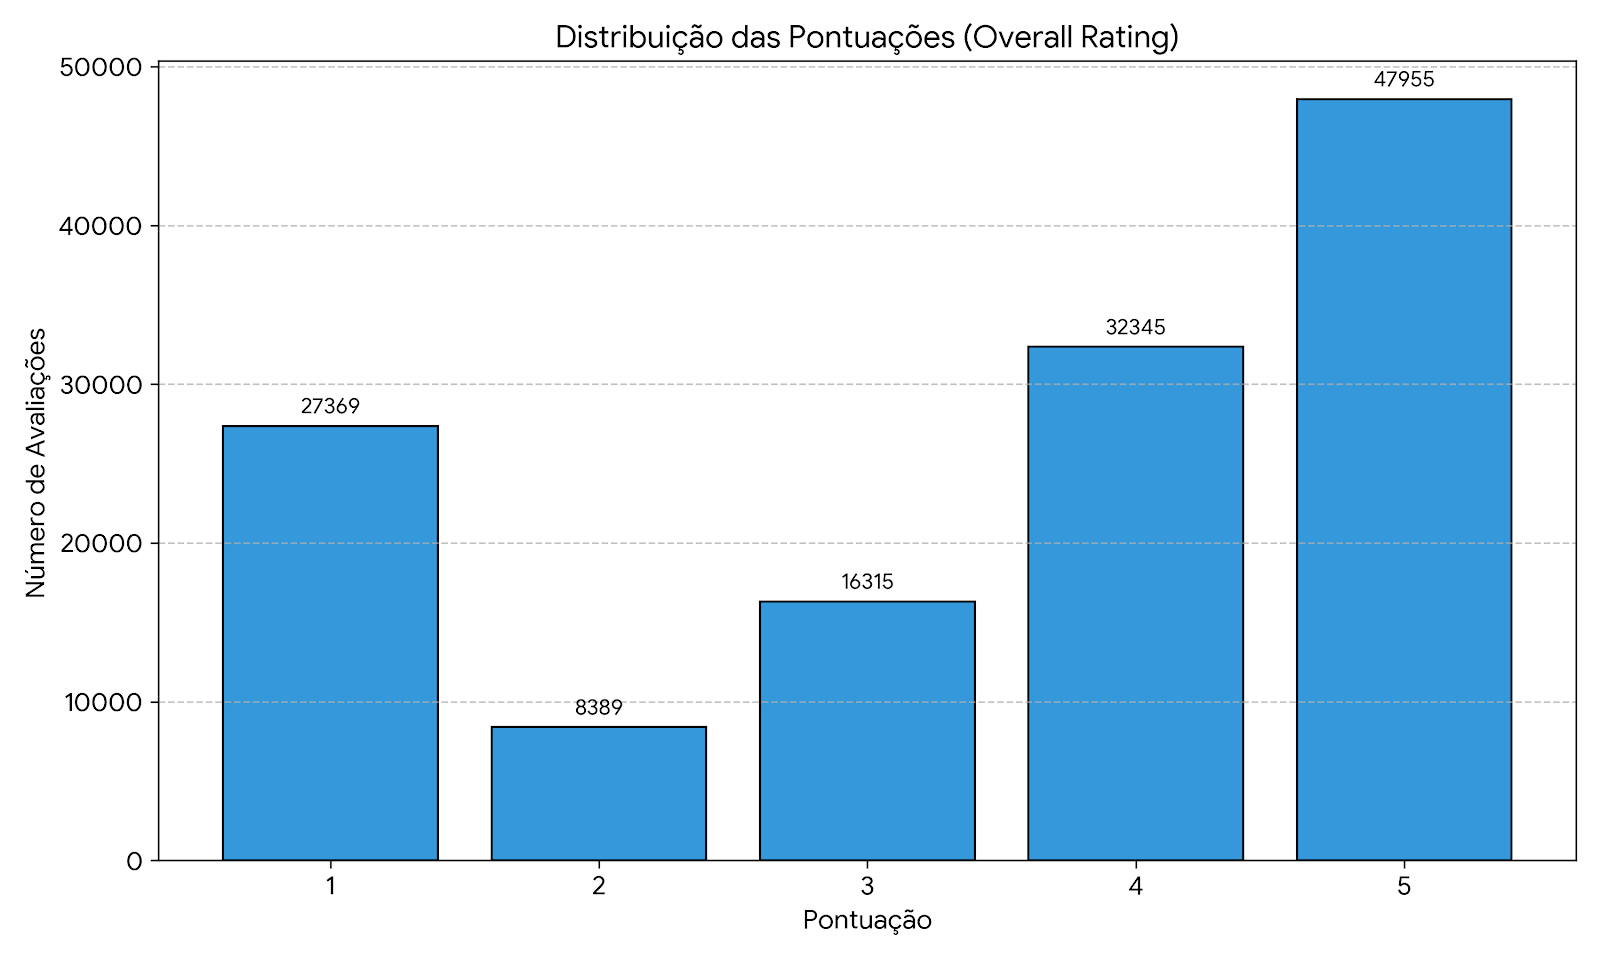
\includegraphics[width=\columnwidth]{figuras/Histograma.png}
    \caption{Distribuição das pontuações (\textit{overall rating}) no corpus B2W-Reviews01. A assimetria entre as notas extremas, com concentração em 1 e 5 estrelas, indica polarização das opiniões dos avaliadores.}
    \label{fig:histograma_ratings}
\end{figure}

Os exemplos da Tabela~\ref{tab:exemplos} ilustram os principais desafios do corpus. No primeiro caso, o texto trata de um problema logístico, devolução de produto avariado, e não de uma opinião sobre o item em si, evidenciando que a polaridade da avaliação pode refletir a experiência de compra e não a qualidade do produto. No segundo, a frustração com a não entrega é reforçada por marcadores de linguagem informal e afetiva (uso excessivo de pontuação e interjeições), fenômeno comum em texto gerado por usuário que desafia modelos baseados em frequência de termos como o TF-IDF. O terceiro caso é o mais crítico para a classificação de sentimentos: o texto é explicitamente negativo, dirigido ao processo de avaliação da plataforma, enquanto a nota e a recomendação são positivas, evidenciando que a polaridade textual nem sempre reflete o sentimento do consumidor sobre o produto~\cite{real2019b2w}.

\begin{table*}[htbp]
    \centering
    \caption{Exemplos de avaliações do corpus B2W-Reviews01}
    \label{tab:exemplos}
    \renewcommand{\arraystretch}{1.4}
    \begin{tabular}{p{0.14\linewidth} p{0.22\linewidth} p{0.38\linewidth} c c}
    \toprule
    \textbf{Produto} & \textbf{Título} & \textbf{Texto} & \textbf{Nota} & \textbf{Recomenda?} \\
    \midrule
    
    Penteadeira JB 7200 com Banqueta Amarelo &
    O produto foi devolvido, devido estar avariado. &
    Gostaria de cancelar esta compra, peço sua gentileza me informar como devo proceder. &
    2 & Não \\
    
    \midrule
    
    Chaleira Elétrica Cadence CEL800 1,7 Litros Inox Prime &
    Eu não recebi o produto????!!!!!!!  &
    Eu não recebi o produto e a americanas sabe disso pois já relatei a reclamação diversas vezes!!! Só vão devolver o dinheiro no procon e isso mesmo????? &
    1 & Não \\
    
    \midrule
    
    Smartphone Multilaser MS80 4G 32GB &
    bom &
    que merda pq n pode so da estrela tem que escrever alguma coisa para avaliar koe americanas muda isso &
    5 & Sim \\
    
    \bottomrule
    \end{tabular}
\end{table*}

A Figura~\ref{fig:palavras_frequentes} sugere um aspecto relevante para o pré-processamento: termos como ``entrega'', ``prazo'' e ``americanas'' figuram entre os mais frequentes, indicando que parte das avaliações pode tratar da experiência de compra e não do produto em si, o que tende a introduzir ruído para a tarefa de classificação de sentimento. A Figura~\ref{fig:categorias_produtos} mostra que o corpus concentra produtos em categorias de eletrônicos, com Celulares e Smartphones representando cerca de 26\% dos produtos únicos. As Figuras~\ref{fig:ranking_categoria} e~\ref{fig:ranking_negativo_categoria}, analisadas em conjunto, indicam que as categorias de maior volume, como Móveis e Beleza e Perfumaria, estão entre as de menor média de rating, ao passo que categorias de nicho como Linha Industrial e Agro, Indústria e Comércio concentram as avaliações mais negativas, apontando para uma distribuição de polaridade heterogênea entre domínios do corpus.

\begin{figure}[htbp]
    \centering
    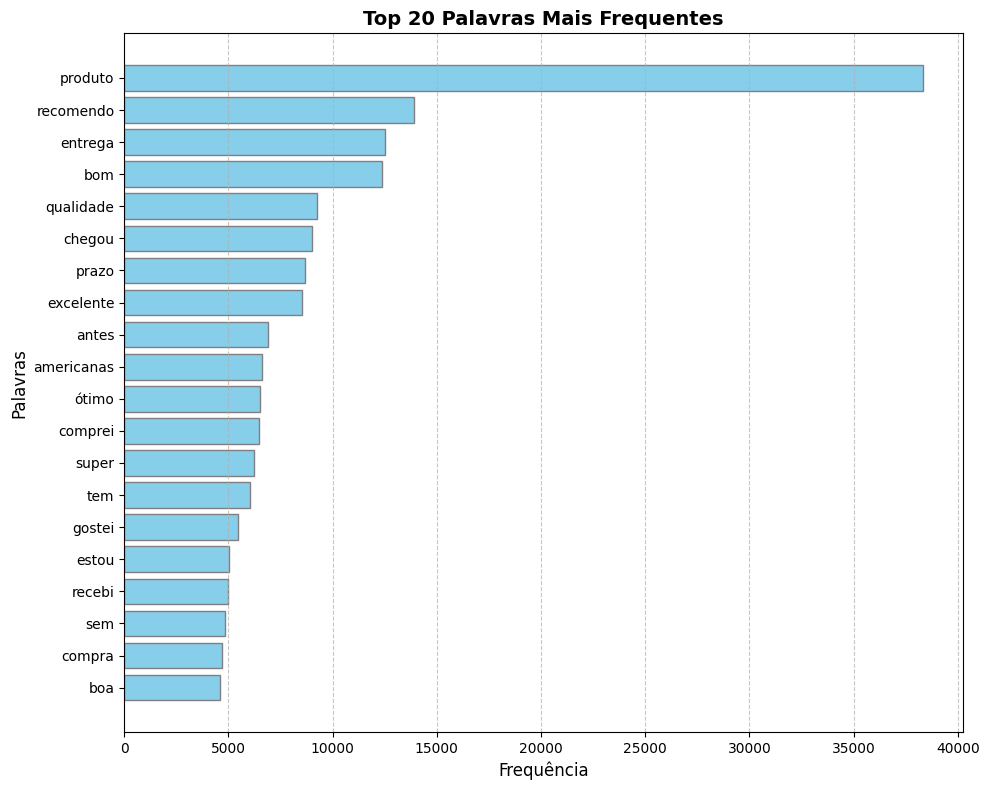
\includegraphics[width=\columnwidth]{figuras/Figura_2.png}
    \caption{Frequência absoluta das 20 palavras mais recorrentes no corpus B2W-Reviews01 após remoção de \textit{stopwords}. A predominância de termos como ``produto'', ``entrega'' e ``prazo'' evidencia que as avaliações cobrem tanto a qualidade do item quanto a experiência de compra.}
    \label{fig:palavras_frequentes}
\end{figure}

\begin{figure}[htbp]
    \centering
    
\includegraphics[width=\columnwidth]{figuras/Figura_3.png}
    \caption{Top 10 categorias de primeiro nível com maior número de produtos únicos no corpus. Móveis lidera as categorias, seguido por Beleza e Perfumaria, com uma diferença muito pequena.}
    \label{fig:categorias_produtos}
\end{figure}

\begin{figure}[htbp]
    \centering
    % 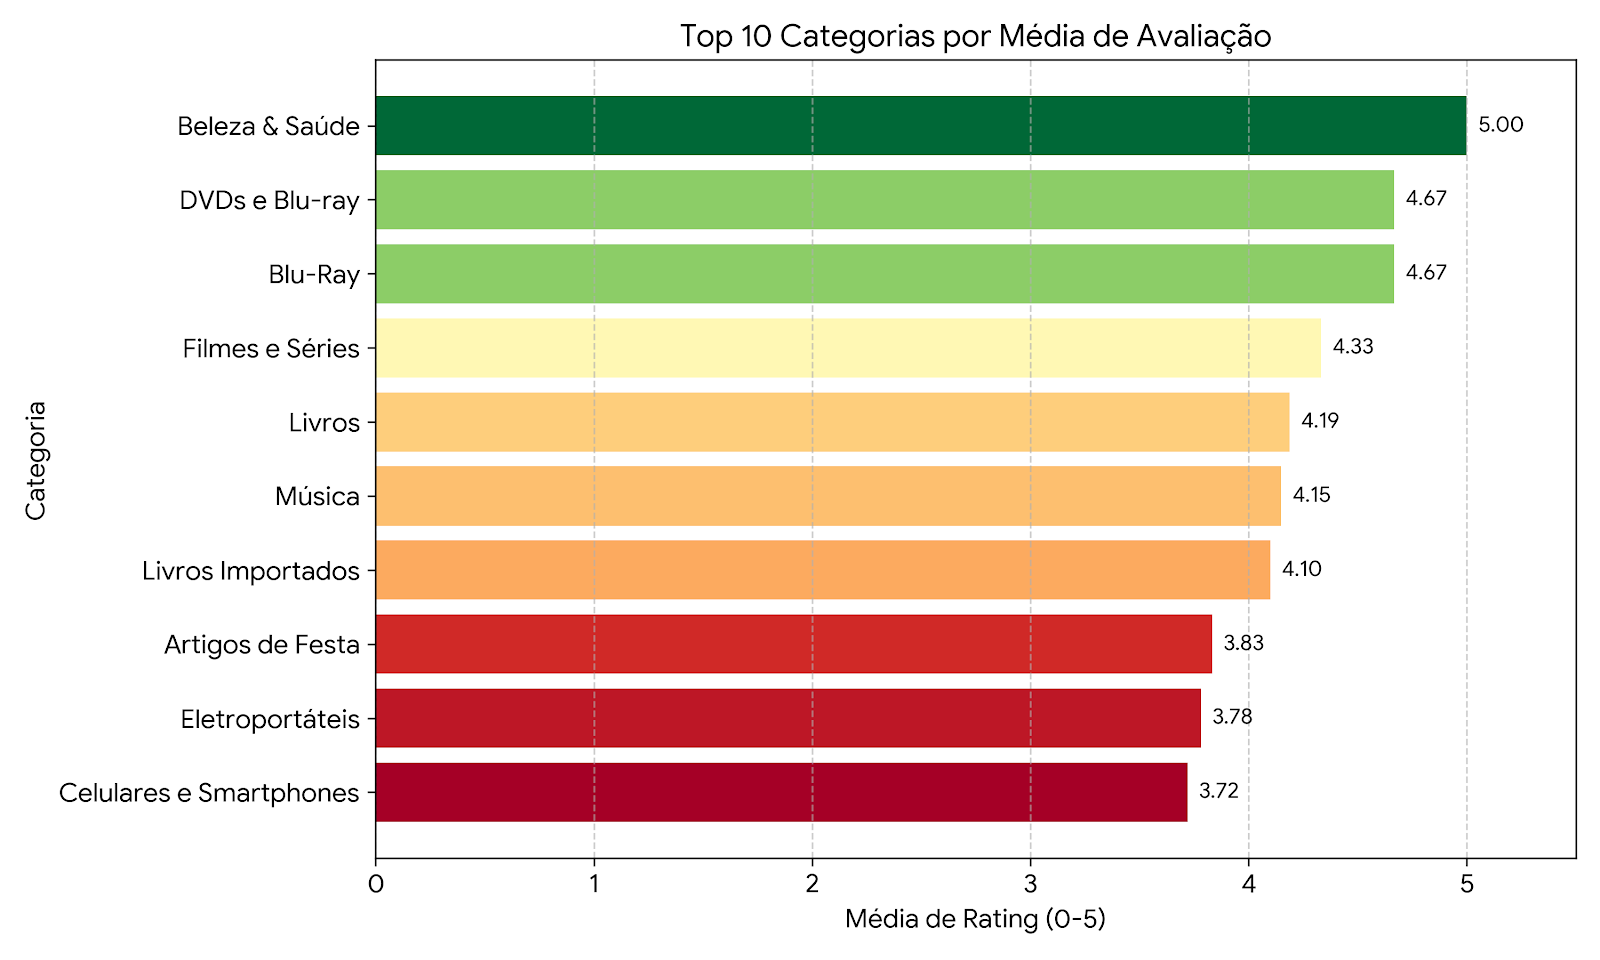
\includegraphics[width=\columnwidth]{figuras/tp_ranking_por_categoria.png}
    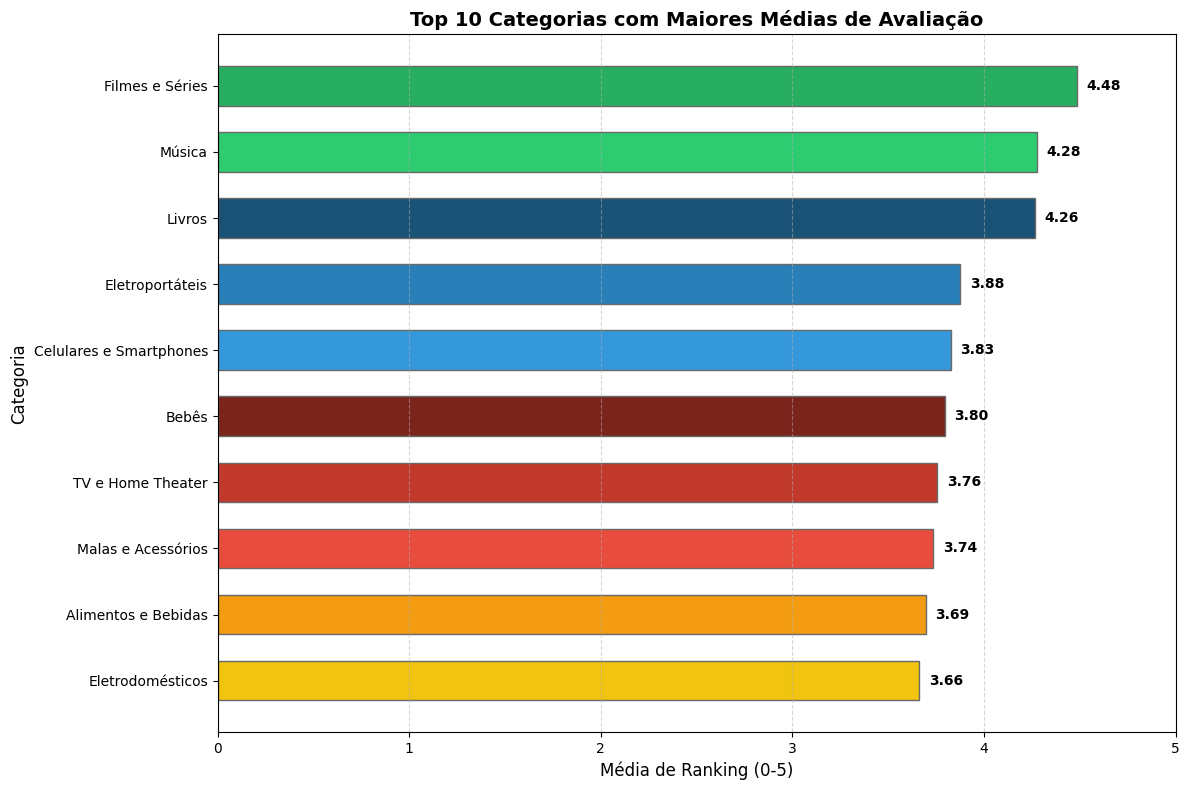
\includegraphics[width=\columnwidth]{figuras/Figura_4.png}
    \caption{Média de avaliação por categoria de produto. Categorias de entretenimento e mídia física (DVDs, Blu-ray, Livros) concentram as maiores médias, enquanto Móveis e Beleza e Perfumaria, categorias com maior volume de avaliações, apresentam as menores médias, sugerindo maior incidência de experiências negativas nesses segmentos.}
    \label{fig:ranking_categoria}
\end{figure}

\begin{figure}[htbp]
    \centering
    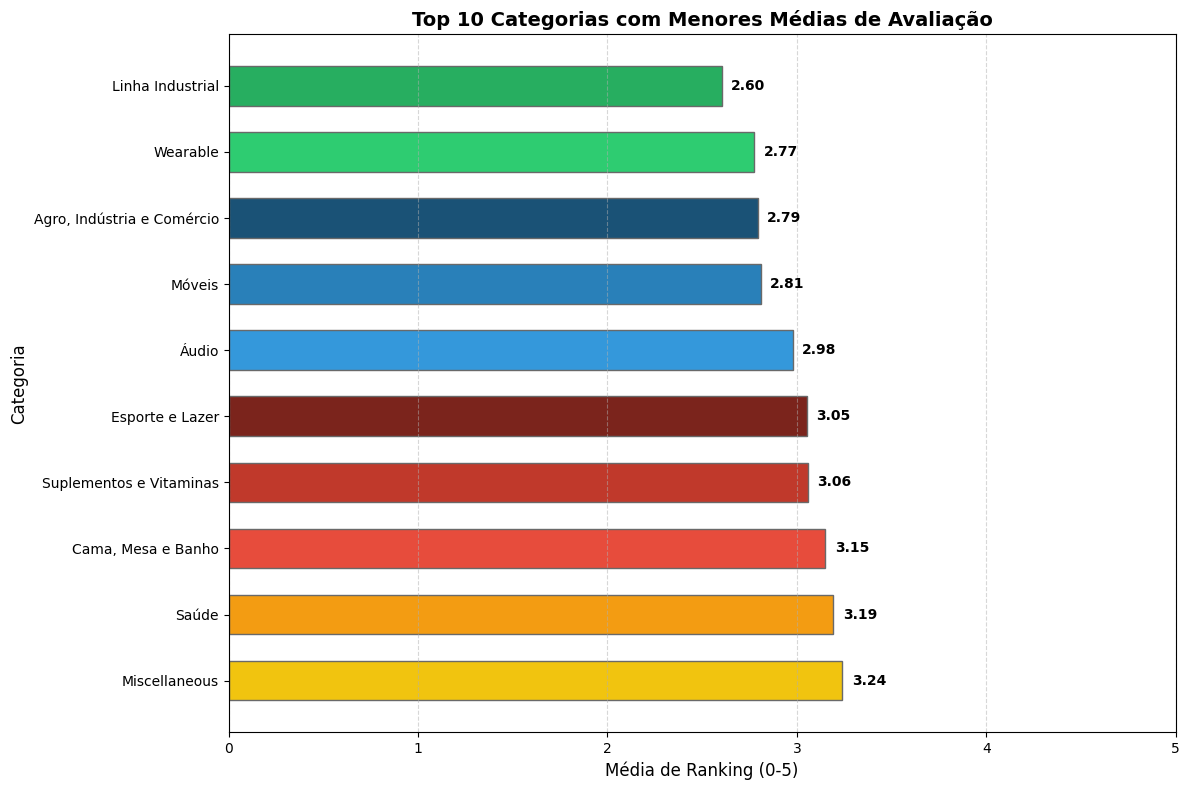
\includegraphics[width=\columnwidth]{figuras/Figura_5.png}
    \caption{Top 10 categorias com menor média de avaliação no corpus. Linha Industrial, Agro, Indústria e Comércio e Sinalização e Segurança concentram as piores médias, todas abaixo de 3,0, sugerindo que categorias de nicho e baixo volume podem apresentar maior proporção de avaliações negativas.}
    \label{fig:ranking_negativo_categoria}
\end{figure}

\begin{figure}[htbp]
    \centering
    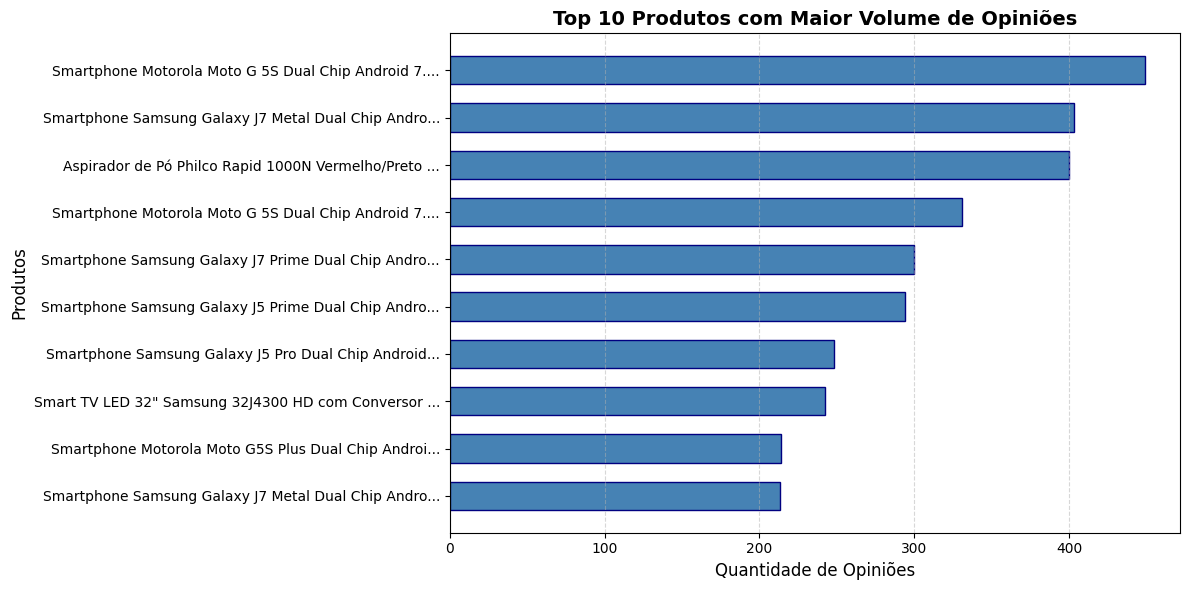
\includegraphics[width=\columnwidth]{figuras/Top 10 Produtos com Maior Volume.png}
    \caption{Top 10 produtos com maior volume de opiniões no corpus. Os celulares são os produtos com maior volume de opiniões.}
     \label{fig:ranking_volume_opinioes}
\end{figure}

 \begin{figure}[htbp]
    \centering
    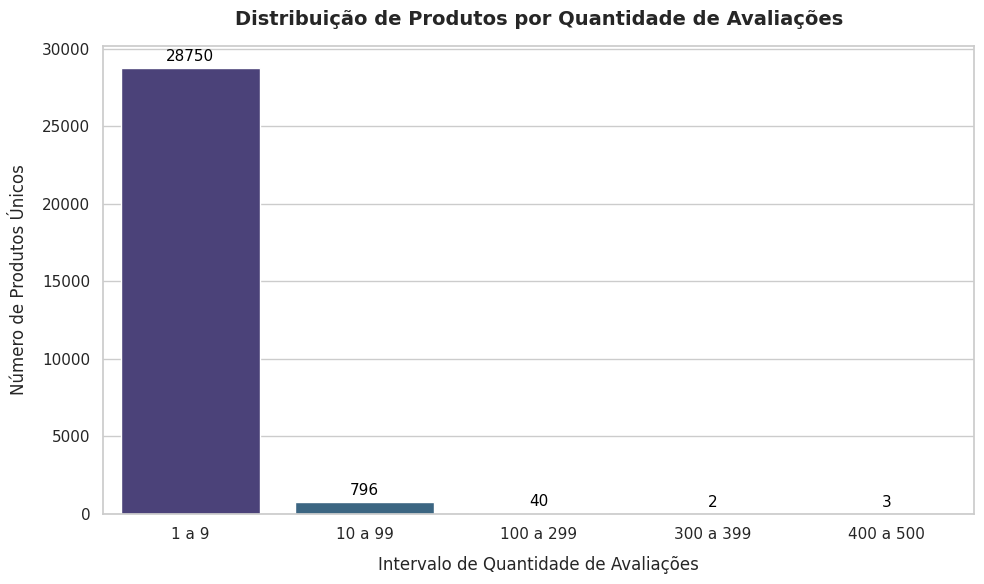
\includegraphics[width=\columnwidth]{figuras/Produtos por Qtde de Avaliacoes.png}
    \caption{Distribuição de produtos pela quantidade de avaliações no corpus. Os produtos podem ter uma ou várias avaliações, temos produtos com 499 avaliações.}
     \label{fig:ranking_volume_opinioes}
\end{figure}

\begin{figure}[htbp]
    \centering
    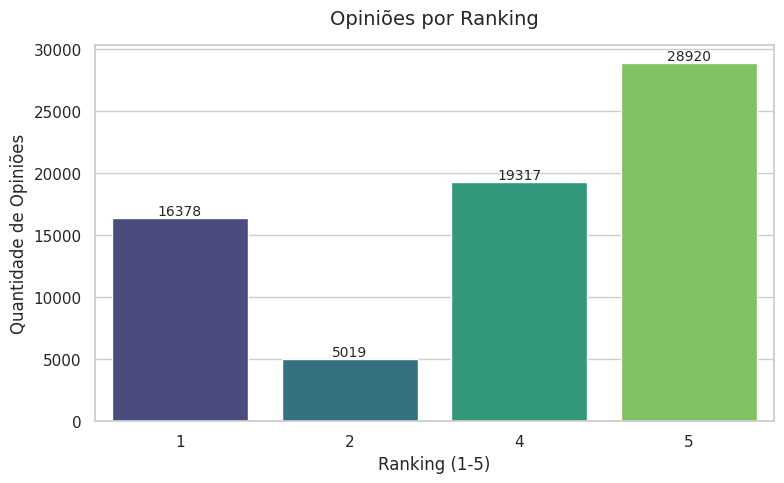
\includegraphics[width=\columnwidth]{figuras/Opinioes por Ranking.png}
    \caption{Distribuição por Ranking de avaliações no corpus. O Ranking se apresenta de 1 até 5. Sendo 1 e 2, avaliações negativas, 3 intermediária e 4 e 5 positivas. }
     \label{fig:ranking_volume_opinioes}
\end{figure}

\begin{figure}[htbp]
    \centering
    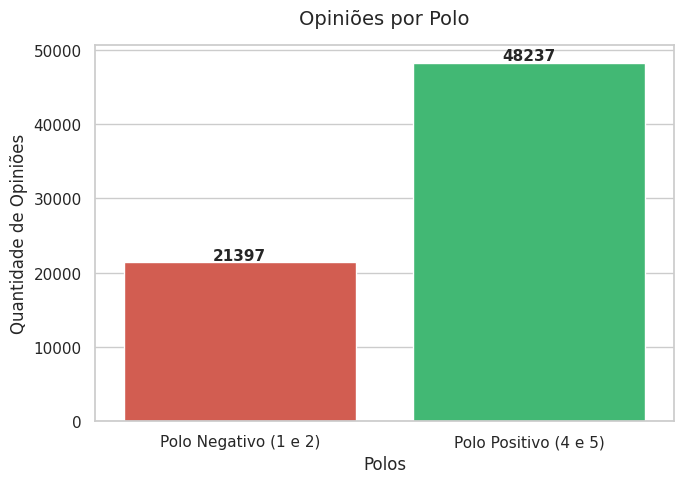
\includegraphics[width=\columnwidth]{figuras/Opiniões por Polo.png}
    \caption{Distribuição de avaliações por polos no corpus. As avaliações 1 e 2 representa o polo negativo e as avaliações 4 e 5, o polo positivo.}
     \label{fig:ranking_volume_opinioes}
\end{figure}

\subsection{Visão Geral dos Pipelines}
\label{subsec:pipelines}

O projeto é composto por dois pipelines principais, apresentados nas Figuras~\ref{fig:pipeline_classification} e \ref{fig:pipeline_recommendation}. O primeiro abrange desde a ingestão dos dados brutos até a seleção do modelo campeão de classificação de sentimento. O segundo consome as saídas do modelo campeão para construir e avaliar o motor de recomendação orientado por sentimento.

\begin{figure}[htbp]
  \centering
  \footnotesize % Fonte reduzida de \small para \footnotesize
  \sffamily
  \setlength{\extrarowheight}{6pt} % Reduzido o espaço extra dentro das células

  \definecolor{colorIngestao}{HTML}{1A4D3E}
  \definecolor{colorRepres}{HTML}{3B2F85}
  \definecolor{colorClassif}{HTML}{5C2A18}
  \definecolor{colorAvaliacao}{HTML}{0F4C81}
  \definecolor{colorSaida}{HTML}{1E5618}
  \definecolor{colorSubtexto}{HTML}{E5E7EB}

  % O resizebox garante que a figura nunca ultrapasse a largura da coluna
  \resizebox{\columnwidth}{!}{%
  \begin{tabular}{c}

    % Aumentado o p{} para 7.5cm para forçar o texto a usar menos linhas
    \begin{tabular}{|p{7.5cm}|}
      \hline
      \rowcolor{colorIngestao}
      \centering \textcolor{white}{\textbf{Corpus B2W-Reviews01}} \tabularnewline
      \rowcolor{colorIngestao}
      \centering \textcolor{colorSubtexto}{\scriptsize Avaliações brutas em português brasileiro} \tabularnewline
      \hline
    \end{tabular} \\[-1ex] % [-1ex] aproxima a seta da caixa superior
    $\downarrow$ \\[-1ex] % [-1ex] aproxima a seta da caixa inferior

    \begin{tabular}{|p{7.5cm}|}
      \hline
      \rowcolor{colorIngestao}
      \centering \textcolor{white}{\textbf{Mapeamento de Polaridade}} \tabularnewline
      \rowcolor{colorIngestao}
      \centering \textcolor{colorSubtexto}{\scriptsize Notas 1--2: negativo $\cdot$ Notas 4--5: positivo $\cdot$ Nota 3: descartada} \tabularnewline
      \hline
    \end{tabular} \\[-1ex]
    $\downarrow$ \\[-1ex]

    \begin{tabular}{|p{7.5cm}|}
      \hline
      \rowcolor{colorIngestao}
      \centering \textcolor{white}{\textbf{Análise Exploratória (EDA)}} \tabularnewline
      \rowcolor{colorIngestao}
      \centering \textcolor{colorSubtexto}{\scriptsize Distribuição de classes, dados faltantes e estatísticas} \tabularnewline
      \hline
    \end{tabular} \\[-1ex]
    $\downarrow$ \\[-1ex]

    \begin{tabular}{|p{7.5cm}|}
      \hline
      \rowcolor{colorIngestao}
      \centering \textcolor{white}{\textbf{Balanceamento de Classes}} \tabularnewline
      \rowcolor{colorIngestao}
      \centering \textcolor{colorSubtexto}{\scriptsize Pesos por classe no treinamento} \tabularnewline
      \hline
    \end{tabular} \\[-1ex]
    $\downarrow$ \\[-1ex]

    \begin{tabular}{|p{7.5cm}|}
      \hline
      \rowcolor{colorIngestao}
      \centering \textcolor{white}{\textbf{Divisão Estratificada}} \tabularnewline
      \rowcolor{colorIngestao}
      \centering \textcolor{colorSubtexto}{\scriptsize Treino 60\% $\cdot$ Validação 20\% $\cdot$ Teste 20\%} \tabularnewline
      \hline
    \end{tabular} \\[-1ex]
    $\downarrow$ \\[-1ex]

    \begin{tabular}{|p{7.5cm}|}
      \hline
      \rowcolor{colorIngestao}
      \centering \textcolor{white}{\textbf{Pré-processamento Textual}} \tabularnewline
      \rowcolor{colorIngestao}
      \centering \textcolor{colorSubtexto}{\scriptsize Normalização $\cdot$ tokenização $\cdot$ lematização (TF-IDF)} \tabularnewline
      \hline
    \end{tabular} \\[-1ex]
    $\downarrow$ \\[-1ex]

    \begin{tabular}{|p{7.5cm}|}
      \hline
      \rowcolor{colorRepres}
      \centering \textcolor{white}{\textbf{Representação / Preparação}} \tabularnewline
      \rowcolor{colorRepres}
      \centering \textcolor{white}{\scriptsize $\bullet$ TF-IDF (esparsa) $\quad \bullet$ BERTimbau \texttt{[CLS]} (densa)} \tabularnewline
      \rowcolor{colorRepres}
      \centering \textcolor{white}{\scriptsize $\bullet$ \textit{Prompting} Estruturado (JSON) para LLMs} \tabularnewline
      \hline
    \end{tabular} \\[-1ex]
    $\downarrow$ \\[-1ex]

    \begin{tabular}{|p{7.5cm}|}
      \hline
      \rowcolor{colorClassif}
      \centering \textcolor{white}{\textbf{Modelagem e Inferência}} \tabularnewline
      \rowcolor{colorClassif}
      \centering \textcolor{white}{\scriptsize $\bullet$ Regressão Logística (TF-IDF e BERTimbau)} \tabularnewline
      \rowcolor{colorClassif}
      \centering \textcolor{white}{\scriptsize $\bullet$ Inferência \textit{One-Shot} (Gemma 4 e Qwen 3.5)} \tabularnewline
      \hline
    \end{tabular} \\[-1ex]
    $\downarrow$ \\[-1ex]

    \begin{tabular}{|p{7.5cm}|}
      \hline
      \rowcolor{colorAvaliacao}
      \centering \textcolor{white}{\textbf{Validação Cruzada Estratificada}} \tabularnewline
      \rowcolor{colorAvaliacao}
      \centering \textcolor{colorSubtexto}{\scriptsize TF-IDF: $k=5$ $\cdot$ BERT: $k=3$ (Apenas supervisionados)} \tabularnewline
      \hline
    \end{tabular} \\[-1ex]
    $\downarrow$ \\[-1ex]

    \begin{tabular}{|p{7.5cm}|}
      \hline
      \rowcolor{colorAvaliacao}
      \centering \textcolor{white}{\textbf{Avaliação Quantitativa (Teste)}} \tabularnewline
      \rowcolor{colorAvaliacao}
      \centering \textcolor{white}{\scriptsize $\bullet$ F1-macro $\quad$ $\bullet$ AUC-ROC} \tabularnewline
      \rowcolor{colorAvaliacao}
      \centering \textcolor{white}{\scriptsize $\bullet$ Precisão $\quad$ $\bullet$ Revocação $\quad$ $\bullet$ Matriz de Confusão} \tabularnewline
      \hline
    \end{tabular} \\[-1ex]
    $\downarrow$ \\[-1ex]

    \begin{tabular}{|p{7.5cm}|}
      \hline
      \rowcolor{colorAvaliacao}
      \centering \textcolor{white}{\textbf{Avaliação Qualitativa}} \tabularnewline
      \rowcolor{colorAvaliacao}
      \centering \textcolor{colorSubtexto}{\scriptsize Inspeção manual (90 instâncias) $\cdot$ Kappa de Cohen} \tabularnewline
      \hline
    \end{tabular} \\[-1ex]
    $\downarrow$ \\[-1ex]

    \begin{tabular}{|p{7.5cm}|}
      \hline
      \rowcolor{colorSaida}
      \centering \textcolor{white}{\textbf{Seleção do Modelo Campeão}} \tabularnewline
      \rowcolor{colorSaida}
      \centering \textcolor{colorSubtexto}{\scriptsize Melhor F1-macro no conjunto de teste} \tabularnewline
      \hline
    \end{tabular} \\
    \medskip \\ % Espaço reduzido antes da legenda

    % Legenda otimizada
    \begin{tabular}{ll}
      \fcolorbox{black}{colorIngestao}{\rule{0pt}{4pt}\rule{4pt}{0pt}} \scriptsize Ingestão e Preparação & 
      \fcolorbox{black}{colorRepres}{\rule{0pt}{4pt}\rule{4pt}{0pt}} \scriptsize Representação / Prompt \\
      \fcolorbox{black}{colorClassif}{\rule{0pt}{4pt}\rule{4pt}{0pt}} \scriptsize Modelagem / Inferência & 
      \fcolorbox{black}{colorAvaliacao}{\rule{0pt}{4pt}\rule{4pt}{0pt}} \scriptsize Avaliação \\
      \fcolorbox{black}{colorSaida}{\rule{0pt}{4pt}\rule{4pt}{0pt}} \scriptsize Saída & \\
    \end{tabular}

  \end{tabular}%
  } % Fechamento do resizebox
  \caption{Pipeline de classificação de sentimento sobre o corpus B2W-Reviews01, contemplando o treinamento dos modelos supervisionados e a inferência direta via LLMs até a seleção do modelo campeão.}
  \label{fig:pipeline_classification}
\end{figure}
% \begin{figure}[htbp]
%   \centering
%   \small
%   \sffamily
%   \setlength{\extrarowheight}{3pt}

%   \definecolor{colorIngestao}{HTML}{1A4D3E}
%   \definecolor{colorRepres}{HTML}{3B2F85}
%   \definecolor{colorClassif}{HTML}{5C2A18}
%   \definecolor{colorAvaliacao}{HTML}{0F4C81}
%   \definecolor{colorSaida}{HTML}{1E5618}
%   \definecolor{colorSubtexto}{HTML}{E5E7EB}

%   \begin{tabular}{c}

%     \begin{tabular}{|p{5.5cm}|}
%       \hline
%       \rowcolor{colorIngestao}
%       \centering \textcolor{white}{\textbf{Corpus B2W-Reviews01}} \tabularnewline
%       \rowcolor{colorIngestao}
%       \centering \textcolor{colorSubtexto}{\footnotesize Avaliações brutas em português brasileiro} \tabularnewline
%       \hline
%     \end{tabular} \\
%     $\downarrow$ \\

%     \begin{tabular}{|p{5.5cm}|}
%       \hline
%       \rowcolor{colorIngestao}
%       \centering \textcolor{white}{\textbf{Mapeamento de Polaridade}} \tabularnewline
%       \rowcolor{colorIngestao}
%       \centering \textcolor{colorSubtexto}{\footnotesize Notas 1--2: negativo $\cdot$ Notas 4--5: positivo $\cdot$ Nota 3: descartada} \tabularnewline
%       \hline
%     \end{tabular} \\
%     $\downarrow$ \\

%     \begin{tabular}{|p{5.5cm}|}
%       \hline
%       \rowcolor{colorIngestao}
%       \centering \textcolor{white}{\textbf{Análise Exploratória (EDA)}} \tabularnewline
%       \rowcolor{colorIngestao}
%       \centering \textcolor{colorSubtexto}{\footnotesize Distribuição de classes, dados faltantes e estatísticas} \tabularnewline
%       \hline
%     \end{tabular} \\
%     $\downarrow$ \\

%     \begin{tabular}{|p{5.5cm}|}
%       \hline
%       \rowcolor{colorIngestao}
%       \centering \textcolor{white}{\textbf{Balanceamento de Classes}} \tabularnewline
%       \rowcolor{colorIngestao}
%       \centering \textcolor{colorSubtexto}{\footnotesize Pesos por classe no treinamento} \tabularnewline
%       \hline
%     \end{tabular} \\
%     $\downarrow$ \\

%     \begin{tabular}{|p{5.5cm}|}
%       \hline
%       \rowcolor{colorIngestao}
%       \centering \textcolor{white}{\textbf{Divisão Estratificada}} \tabularnewline
%       \rowcolor{colorIngestao}
%       \centering \textcolor{colorSubtexto}{\footnotesize Treino 70\% $\cdot$ Validação 15\% $\cdot$ Teste 15\%} \tabularnewline
%       \hline
%     \end{tabular} \\
%     $\downarrow$ \\

%     \begin{tabular}{|p{5.5cm}|}
%       \hline
%       \rowcolor{colorIngestao}
%       \centering \textcolor{white}{\textbf{Pré-processamento Textual}} \tabularnewline
%       \rowcolor{colorIngestao}
%       \centering \textcolor{colorSubtexto}{\footnotesize Normalização $\cdot$ tokenização $\cdot$ lematização (TF-IDF)} \tabularnewline
%       \hline
%     \end{tabular} \\
%     $\downarrow$ \\

%     \begin{tabular}{|p{5.5cm}|}
%       \hline
%       \rowcolor{colorRepres}
%       \centering \textcolor{white}{\textbf{Representação da Informação}} \tabularnewline
%       \rowcolor{colorRepres}
%       \centering \textcolor{white}{\footnotesize $\bullet$ TF-IDF (uni e bigramas)} \tabularnewline
%       \rowcolor{colorRepres}
%       \centering \textcolor{white}{\footnotesize $\bullet$ BERTimbau \texttt{[CLS]} (pesos congelados)} \tabularnewline
%       % \rowcolor{colorRepres}
%       % \centering \textcolor{white}{\footnotesize $\bullet$ BERTimbau fine-tuning} \tabularnewline
%       \hline
%     \end{tabular} \\
%     $\downarrow$ \\

%     \begin{tabular}{|p{5.5cm}|}
%       \hline
%       \rowcolor{colorClassif}
%       \centering \textcolor{white}{\textbf{Treinamento dos Modelos}} \tabularnewline
%       \rowcolor{colorClassif}
%       \centering \textcolor{white}{\footnotesize $\bullet$ TF-IDF + Regressão Logística} \tabularnewline
%       \rowcolor{colorClassif}
%       \centering \textcolor{white}{\footnotesize $\bullet$ BERTimbau + Regressão Logística} \tabularnewline
%       % \rowcolor{colorClassif}
%       % \centering \textcolor{white}{\footnotesize $\bullet$ BERTimbau fine-tuning + MLP} \tabularnewline
%       \hline
%     \end{tabular} \\
%     $\downarrow$ \\

%     \begin{tabular}{|p{5.5cm}|}
%       \hline
%       \rowcolor{colorAvaliacao}
%       \centering \textcolor{white}{\textbf{Validação Cruzada Estratificada}} \tabularnewline
%       \rowcolor{colorAvaliacao}
%       \centering \textcolor{colorSubtexto}{\footnotesize TF-IDF: $k=5$ com Grid Search $\cdot$ BERTimbau: $k=3$} \tabularnewline
%       \hline
%     \end{tabular} \\
%     $\downarrow$ \\

%     \begin{tabular}{|p{5.5cm}|}
%       \hline
%       \rowcolor{colorAvaliacao}
%       \centering \textcolor{white}{\textbf{Avaliação Quantitativa}} \tabularnewline
%       \rowcolor{colorAvaliacao}
%       \centering \textcolor{white}{\footnotesize $\bullet$ F1-macro $\quad$ $\bullet$ AUC-ROC} \tabularnewline
%       \rowcolor{colorAvaliacao}
%       \centering \textcolor{white}{\footnotesize $\bullet$ Precisão $\quad$ $\bullet$ Revocação $\quad$ $\bullet$ Matriz de Confusão} \tabularnewline
%       \hline
%     \end{tabular} \\
%     $\downarrow$ \\

%     \begin{tabular}{|p{5.5cm}|}
%       \hline
%       \rowcolor{colorAvaliacao}
%       \centering \textcolor{white}{\textbf{Avaliação Qualitativa}} \tabularnewline
%       \rowcolor{colorAvaliacao}
%       \centering \textcolor{colorSubtexto}{\footnotesize Inspeção manual (90 instâncias) $\cdot$ Kappa de Cohen} \tabularnewline
%       \hline
%     \end{tabular} \\
%     $\downarrow$ \\

%     \begin{tabular}{|p{5.5cm}|}
%       \hline
%       \rowcolor{colorSaida}
%       \centering \textcolor{white}{\textbf{Seleção do Modelo Campeão}} \tabularnewline
%       \rowcolor{colorSaida}
%       \centering \textcolor{colorSubtexto}{\footnotesize Melhor F1-macro no conjunto de teste} \tabularnewline
%       \hline
%     \end{tabular} \\
%     \bigskip \\

%     \begin{tabular}{lll}
%       \fcolorbox{black}{colorIngestao}{\rule{0pt}{4pt}\rule{4pt}{0pt}} \footnotesize Ingestão e Preparação &
%       \fcolorbox{black}{colorRepres}{\rule{0pt}{4pt}\rule{4pt}{0pt}} \footnotesize Representação &
%       \fcolorbox{black}{colorClassif}{\rule{0pt}{4pt}\rule{4pt}{0pt}} \footnotesize Modelagem \\
%       \fcolorbox{black}{colorAvaliacao}{\rule{0pt}{4pt}\rule{4pt}{0pt}} \footnotesize Avaliação &
%       \fcolorbox{black}{colorSaida}{\rule{0pt}{4pt}\rule{4pt}{0pt}} \footnotesize Saída &
%     \end{tabular}

%   \end{tabular}
%   \caption{Pipeline de classificação de sentimento sobre o corpus B2W-Reviews01, desde a ingestão dos dados brutos até a seleção do modelo campeão.}
%   \label{fig:pipeline_classification}
% \end{figure}

\begin{figure}[htbp]
  \centering
  \small
  \sffamily
  \setlength{\extrarowheight}{3pt}

  \definecolor{colorIngestao}{HTML}{1A4D3E}
  \definecolor{colorRepres}{HTML}{3B2F85}
  \definecolor{colorClassif}{HTML}{5C2A18}
  \definecolor{colorAvaliacao}{HTML}{0F4C81}
  \definecolor{colorSaida}{HTML}{1E5618}
  \definecolor{colorSubtexto}{HTML}{E5E7EB}

  \begin{tabular}{c}

    \begin{tabular}{|p{6.0cm}|}
      \hline
      \rowcolor{colorIngestao}
      \centering \textcolor{white}{\textbf{Classificação do Corpus Completo}} \tabularnewline
      \rowcolor{colorIngestao}
      \centering \textcolor{colorSubtexto}{\footnotesize Inferência com modelo campeão (Pipeline 1)} \tabularnewline
      \hline
    \end{tabular} \\
    $\downarrow$ \\

    \begin{tabular}{|p{6.0cm}|}
      \hline
      \rowcolor{colorIngestao}
      \centering \textcolor{white}{\textbf{Score de Sentimento por Produto}} \tabularnewline
      \rowcolor{colorIngestao}
      \centering \textcolor{colorSubtexto}{\footnotesize Proporção de avaliações positivas $\cdot$ mínimo de 5 avaliações} \tabularnewline
      \hline
    \end{tabular} \\
    $\downarrow$ \\

    \begin{tabular}{|p{6.0cm}|}
      \hline
      \rowcolor{colorRepres}
      \centering \textcolor{white}{\textbf{Vetorização dos Títulos}} \tabularnewline
      \rowcolor{colorRepres}
      \centering \textcolor{white}{\footnotesize Serafim PT* (335M) $\cdot$ mean pooling $\cdot$ 1024 dimensões} \tabularnewline
      \hline
    \end{tabular} \\
    $\downarrow$ \\

    \begin{tabular}{|p{6.0cm}|}
      \hline
      \rowcolor{colorClassif}
      \centering \textcolor{white}{\textbf{Indexação em Banco Vetorial}} \tabularnewline
      \rowcolor{colorClassif}
      \centering \textcolor{colorSubtexto}{\footnotesize FAISS $\cdot$ ChromaDB $\cdot$ Qdrant (a definir)} \tabularnewline
      \hline
    \end{tabular} \\
    $\downarrow$ \\

    \begin{tabular}{|p{6.0cm}|}
      \hline
      \rowcolor{colorClassif}
      \centering \textcolor{white}{\textbf{Busca e Recuperação (ANN)}} \tabularnewline
      \rowcolor{colorClassif}
      \centering \textcolor{colorSubtexto}{\footnotesize Top-K candidatos via similaridade de cosseno} \tabularnewline
      \hline
    \end{tabular} \\
    $\downarrow$ \\

    \begin{tabular}{|p{6.0cm}|}
      \hline
      \rowcolor{colorClassif}
      \centering \textcolor{white}{\textbf{Re-ranqueamento por Sentimento}} \tabularnewline
      \rowcolor{colorClassif}
      \centering \textcolor{colorSubtexto}{\footnotesize Combinação ponderada de similaridade e score de sentimento} \tabularnewline
      \hline
    \end{tabular} \\
    $\downarrow$ \\

    \begin{tabular}{|p{6.0cm}|}
      \hline
      \rowcolor{colorAvaliacao}
      \centering \textcolor{white}{\textbf{Avaliação Quantitativa}} \tabularnewline
      \rowcolor{colorAvaliacao}
      \centering \textcolor{white}{\footnotesize $\bullet$ NDCG@k $\quad$ $\bullet$ Precision@k} \tabularnewline
      \rowcolor{colorAvaliacao}
      \centering \textcolor{white}{\footnotesize $\bullet$ Recall@k $\quad$} \tabularnewline
      \hline
    \end{tabular} \\
    $\downarrow$ \\

    \begin{tabular}{|p{6.0cm}|}
      \hline
      \rowcolor{colorAvaliacao}
      \centering \textcolor{white}{\textbf{Avaliação Qualitativa}} \tabularnewline
      \rowcolor{colorAvaliacao}
      \centering \textcolor{colorSubtexto}{\footnotesize 20 pares consulta-lista $\cdot$ Kappa de Cohen} \tabularnewline
      \hline
    \end{tabular} \\
    $\downarrow$ \\

    \begin{tabular}{|p{6.0cm}|}
      \hline
      \rowcolor{colorSaida}
      \centering \textcolor{white}{\textbf{Lista Final de Recomendações}} \tabularnewline
      \rowcolor{colorSaida}
      \centering \textcolor{colorSubtexto}{\footnotesize Top-k produtos ordenados por relevância semântica e sentimento} \tabularnewline
      \hline
    \end{tabular} \\
    \bigskip \\

    \begin{tabular}{lll}
      \fcolorbox{black}{colorIngestao}{\rule{0pt}{4pt}\rule{4pt}{0pt}} \footnotesize Processamento Inicial &
      \fcolorbox{black}{colorRepres}{\rule{0pt}{4pt}\rule{4pt}{0pt}} \footnotesize Representação &
      \fcolorbox{black}{colorClassif}{\rule{0pt}{4pt}\rule{4pt}{0pt}} \footnotesize Recuperação / Ranking \\
      \fcolorbox{black}{colorAvaliacao}{\rule{0pt}{4pt}\rule{4pt}{0pt}} \footnotesize Avaliação &
      \fcolorbox{black}{colorSaida}{\rule{0pt}{4pt}\rule{4pt}{0pt}} \footnotesize Saída &
    \end{tabular}

  \end{tabular}
  \caption{Pipeline de recomendação orientada por sentimento, consumindo as saídas do modelo campeão para construir e avaliar o motor de recuperação e re-ranqueamento.}
  \label{fig:pipeline_recommendation}
\end{figure}


% \begin{figure}[htbp]
%   \centering
%   \fbox{\parbox{0.9\linewidth}{\centering
%     \textit{[Ver Figura separada: Pipeline de Recomendação]}\\
%     {\footnotesize Diagrama gerado como artefato complementar}
%   }}
%   \caption{Pipeline de Recomendação Orientada por Sentimento (Pipeline 2).}
%   \label{fig:pipeline_recommendation}
% \end{figure}

\subsection{Pipeline 1 -- Classificação de Sentimento}
\label{subsec:pipeline1}

\subsubsection{Divisão dos Dados}
\label{subsubsec:split}

Os dados serão divididos em três partições estratificadas por classe de sentimento:

\begin{itemize}[noitemsep]
  \item \textbf{Treino}: 60\% dos dados.
  \item \textbf{Validação}: 20\% dos dados (ajuste de hiperparâmetros).
  \item \textbf{Teste}: 20\% dos dados (avaliação final, utilizado apenas uma vez).
\end{itemize}

A estratificação garante que a proporção de classes positivas e negativas seja preservada em cada partição.

\subsubsection{Pré-processamento Textual}
\label{subsubsec:preprocessing}

A entrada dos modelos será o campo \texttt{review\_text} concatenado ao campo \texttt{review\_title}. O pré-processamento segue as etapas descritas a seguir, calibradas conforme o tipo de representação utilizada.

\paragraph{Normalização textual (aplicada a ambas as representações)}
\begin{enumerate}[noitemsep]
  \item Conversão para minúsculas (\textit{lowercasing}).
  \item Remoção de HTML tags, URLs e caracteres especiais não-alfanuméricos.
  \item Normalização de acentuação e caracteres Unicode (NFD/NFC).
  \item Remoção de espaços duplicados e linhas vazias.
\end{enumerate}

\paragraph{Pré-processamento adicional para TF-IDF (representação esparsa):}
\begin{enumerate}[noitemsep]
  \item Tokenização por espaço e pontuação.
  \item Remoção de \textit{stopwords} em português (lista NLTK).
  \item Lematização com spaCy.
  \item Construção do vocabulário e aplicação do TF-IDF com n-gramas de 1 a 2 (\textit{unigrams} e \textit{bigrams}). A inclusão de bigramas permite capturar associações locais entre termos adjacentes relevantes para o domínio, como ``não recebi'', ``boa qualidade'' e ``prazo entrega'', que perdem seu sentido quando analisadas como tokens isolados.
\end{enumerate}

\paragraph{Pré-processamento para Embeddings (representação densa)}
O BERTimbau utiliza seu próprio tokenizador \textit{WordPiece}, que lida internamente com vocabulário, subpalavras e tokens especiais ([CLS], [SEP]). Para este modelo, aplica-se apenas a normalização textual básica, preservando a estrutura morfológica necessária para o modelo contextual.

\subsubsection{Representação da Informação}
\label{subsubsec:representation}

% \paragraph{Estratégia 1 -- TF-IDF (linha de base esparsa):}
% Será construída uma matriz TF-IDF com os termos mais frequentes, aplicando suavização logarítmica no cálculo do IDF para lidar com termos raros. A ponderação TF-IDF é definida pela equação:


% \begin{equation}
%   \text{TF-IDF}(t,d,D) = \text{TF}(t,d) \times \log\!\left(\frac{N}{n_t}\right)
%   \label{eq:tfidf}
% \end{equation}


% onde $N$ é o total de documentos e $n_t$ é o número de documentos que contêm o termo $t$.

\paragraph{Estratégia 1 -- Linha de Base (\textit{Baseline}) com TF-IDF:}
Como modelo de referência esparso, adotou-se um \textit{pipeline} composto por extração de características via TF-IDF acoplado a um classificador linear. Após a etapa de lematização, os textos foram mapeados para um espaço vetorial limitando-se o vocabulário às 50.000 características (\textit{features}) mais frequentes. Com o intuito de avaliar a influência do contexto local na captura do sentimento, a vetorização foi submetida a uma análise de ablação através de três estratégias de extração: (i) estritamente unigramas, (ii) estritamente bigramas, e (iii) a combinação de unigramas e bigramas.

Para a ponderação dos termos, utilizou-se o fator de suavização logarítmica padrão (com adição de constante para evitar divisões por zero e ignorar termos ausentes), definido pela Equação \ref{eq:tfidf_sklearn}:

\begin{equation}
  \text{TF-IDF}(t,d) = \text{tf}(t,d) \times \left( \log\!\left(\frac{1 + N}{1 + n_t}\right) + 1 \right)
  \label{eq:tfidf_sklearn}
\end{equation}

onde $\text{tf}(t,d)$ é a frequência do n-grama $t$ no documento $d$, $N$ denota o número total de amostras no conjunto de treinamento e $n_t$ é a quantidade de amostras que contêm o n-grama $t$. As matrizes esparsas resultantes serviram como entrada para um modelo de Regressão Logística, cujos hiperparâmetros foram otimizados via busca em grade (\textit{Grid Search}) com validação cruzada estratificada.

% \paragraph{Estratégia 2 -- Embeddings com BERTimbau:}
% Utilizaremos o BERTimbau Base \cite{souza2020bertimbau} via Hugging Face. Serão investigadas duas configurações: (a) \textit{feature extraction}, em que os pesos do BERT são congelados e o vetor do token [CLS] é usado como representação de entrada para um classificador externo; e (b) \textit{fine-tuning} completo, em que uma camada linear é adicionada ao [CLS] e toda a rede é ajustada na tarefa de classificação binária.

\paragraph{Estratégia 2 -- Representações Densas com BERTimbau:}
Como alternativa à representação esparsa, explorou-se a modelagem contextual utilizando o modelo pré-treinado BERTimbau Base (\texttt{neuralmind/bert-base-portuguese-cased}) \cite{souza2020bertimbau}, disponibilizado pela biblioteca \textit{Transformers}. Utilizou-se exclusivamente a estratégia de extração de características (\textit{feature extraction}), na qual os parâmetros do modelo de linguagem são mantidos estáticos (\textit{frozen}). A representação vetorial contínua associada ao \textit{token} especial \texttt{[CLS]} foi extraída para cada documento e utilizada como espaço de atributos para o treinamento de um classificador externo de Regressão Logística. A otimização dos hiperparâmetros do classificador ocorreu mediante busca em grade (\textit{Grid Search}) sob validação cruzada estratificada de 3 vias ($k=3$), incorporando o balanceamento de pesos de classe para atenuar a assimetria dos dados.



\subsubsection{Modelos de Classificação}
\label{subsubsec:classifiers}

Para cada representação, serão treinados os seguintes modelos:

\begin{itemize}[noitemsep]
  \item \textbf{TF-IDF + RL}: linha de base com representação esparsa e classificador linear.
  \item \textbf{BERTimbau + RL}: embedding contextual \texttt{[CLS]} com pesos congelados e classificador linear.
  % \item \textbf{BERTimbau fine-tuning + MLP}: encoder ajustado à tarefa com classificador não-linear treinado ponta-a-ponta.
\end{itemize}

 

\subsubsection{Modelos de Linguagem de Pequena Escala}

Em complemento às abordagens de aprendizado supervisionado (Regressão Logística com TF-IDF e BERTimbau), foram incluídos neste estudo dois Modelos de Linguagem de Grande Escala (LLMs) abertos para atuarem como classificadores baseados em \textit{prompting}. Esses modelos operam sem qualquer atualização de parâmetros, realizando a inferência a partir do contexto injetado como texto de instrução de sistema (\textit{System Prompt}).

Os modelos selecionados para essa etapa foram:

\begin{itemize}
    \item \textbf{Gemma 4-12B QAT}: modelo aberto da família Gemma \cite{gemma_hf_2024}, pré-treinado em dados multilíngues. Utilizou-se a arquitetura de 12 bilhões de parâmetros, associada a técnicas de quantização (\textit{Quantization-Aware Training}) para otimização da inferência computacional.
    \item \textbf{Qwen 3.5-9B}: modelo desenvolvido pela Alibaba Cloud \cite{qwenteam2026qwen35omnitechnicalreport}, reconhecido por seu forte desempenho em tarefas de compreensão semântica multilíngue. Foi adotada a variante estruturada com 9 bilhões de parâmetros.
\end{itemize}


A estratégia de classificação adotou o paradigma \textit{one-shot}, no qual o modelo recebe um texto de configuração de sistema (\textit{system prompt}) contendo diretrizes rígidas sobre a tarefa de análise de sentimento binária, regras para casos ambíguos e um único exemplo prático de entrada e saída esperada. Para garantir a viabilidade da extração sistemática dos resultados, os LLMs foram instruídos a gerar suas respostas exclusivamente no formato de um objeto JSON estruturado. O detalhamento do \textit{prompt} submetido aos modelos é apresentado no Código \ref{lst:prompt-one-shot}.

\lstdefinelanguage{yaml}{
  keywords={task,description,system_prompt,user_template,response_schema,
    type,properties,sentiment,enum,required,additionalProperties,object,string},
  keywordstyle=\color{blue!70!black}\bfseries,
  comment=[l]{\#},
  commentstyle=\color{gray},
  stringstyle=\color{teal},
  morestring=[b]",
  basicstyle=\ttfamily\small,
  breaklines=true,
  literate=%
    {á}{{\'a}}1 {é}{{\'e}}1 {í}{{\'i}}1 {ó}{{\'o}}1 {ú}{{\'u}}1
    {â}{{\^a}}1 {ê}{{\^e}}1 {ô}{{\^o}}1 {ã}{{\~a}}1 {õ}{{\~o}}1
    {ç}{{\c c}}1 {Á}{{\'A}}1 {É}{{\'E}}1 {Ó}{{\'O}}1 {Ã}{{\~A}}1
}

\begin{lstlisting}[language=yaml,caption={Prompt one-shot para classificação binária de sentimento.},label={lst:prompt-one-shot}]
task: sentiment_binary_classification
description: >
  Classificação binária de sentimento (positivo/negativo) de avaliações de
  produtos em português brasileiro (corpus B2W-Reviews01), via prompting
  one-shot (um único exemplo embutido no prompt de sistema, sem treino).

system_prompt: |
  Você é um classificador de sentimento especializado em avaliações de
  e-commerce em português brasileiro. Leia o título e o texto de uma
  avaliação de produto e decida se o cliente está SATISFEITO (positivo)
  ou INSATISFEITO (negativo) com o produto.

  Regras:
  - Responda apenas com o rótulo de sentimento, seguindo exatamente o
    schema JSON solicitado, sem texto adicional.
  - Use "positive" quando a avaliação expressa satisfação, aprovação ou
    recomendação do produto.
  - Use "negative" quando a avaliação expressa insatisfação, reclamação,
    defeito, atraso na entrega ou arrependimento da compra.
  - Baseie-se apenas no conteúdo textual da avaliação (título + texto),
    não em suposições externas.
  - Não existe categoria neutra: escolha sempre "positive" ou "negative",
    mesmo em casos ambíguos, com base no tom predominante do texto.

  Exemplo:
  Título: "Ótimo custo-benefício"
  Texto: "Produto chegou antes do prazo, embalagem intacta e funciona
  perfeitamente. Recomendo a compra."
  Resposta esperada: {"sentiment": "positive"}

user_template: |
  Título: "{title}"
  Texto: "{text}"

response_schema:
  type: object
  properties:
    sentiment:
      type: string
      enum:
        - positive
        - negative
  required:
    - sentiment
  additionalProperties: false
\end{lstlisting}

\subsubsection{Validação e Seleção do Modelo}
\label{subsubsec:validation}
Todos os modelos serão avaliados com validação cruzada estratificada sobre o conjunto de treino e validação, garantindo comparabilidade entre as configurações. Para os modelos baseados em TF-IDF, serão utilizados $k=5$ \textit{folds} com otimização de hiperparâmetros via \textit{Grid Search}. Para o modelo BERTimbau, dado o maior custo computacional, serão utilizados $k=3$ \textit{folds}. Em ambos os casos, o modelo com melhor F1-macro médio entre os \textit{folds} será selecionado para avaliação final no conjunto de teste.

\subsubsection{Métricas de Avaliação -- Classificação}
\label{subsubsec:metrics_classification}

As métricas utilizadas para avaliar os modelos de classificação de sentimento são:

\begin{itemize}[noitemsep]
  \item \textbf{Precisão (P)}: proporção de predições positivas corretas.
  \item \textbf{Revocação (R)}: proporção de positivos verdadeiros recuperados.
  \item \textbf{F1-score macro}: média harmônica de P e R, calculada por classe e depois com média macro (sem ponderação por frequência de classe), definida como:
    \begin{equation}
      F_1 = \frac{2 \cdot P \cdot R}{P + R}
      \label{eq:f1}
    \end{equation}
  \item \textbf{AUC-ROC}: área sob a curva ROC, medida de discriminação do modelo independente do limiar de decisão.
  \item \textbf{Matriz de confusão}: análise qualitativa dos tipos de erro (falsos positivos e falsos negativos).
\end{itemize}

\subsubsection{Avaliação Qualitativa}
\label{subsubsec:qual_classification}

Uma amostra aleatória estratificada de 50 instâncias do conjunto de teste será avaliada manualmente por pelo menos dois integrantes do grupo, de forma independente, quanto à polaridade real do texto. Os rótulos humanos serão comparados aos rótulos automáticos do modelo campeão. Será calculado o coeficiente de concordância Kappa de Cohen entre os avaliadores humanos.

\subsection{Pipeline 2 -- Recomendação Orientada por Sentimento}
\label{subsec:pipeline2}

\subsubsection{Score de Sentimento por Produto}
\label{subsubsec:sentiment_score}

O modelo campeão da etapa de classificação (BERTimbau + RL),
Seção~\ref{subsec:pipeline1}) foi aplicado a todas as avaliações do corpus (splits
de validação e teste, sem uso de dados de treino) para classificá-las como
positivas ou negativas. Para cada produto único (identificado pelo
\texttt{product\_id}), calcula-se um \textit{score} de relevância $S(p)$ definido
como:

\begin{equation}
  S(p) = \frac{|\{\text{avaliações positivas de } p\}|}{|\{\text{todas as avaliações de } p\}|}
  \label{eq:score}
\end{equation}


\subsubsection{Vetorização dos Títulos de Produtos}
\label{subsubsec:vectorization}

Os títulos de produto (\texttt{product\_name}) são vetorizados com o
\textbf{Qwen3-Embedding-0.6B} \cite{qwen3embedding}, um \textit{sentence encoder} multilíngue que produz vetores densos de 1024 dimensões, normalizados em norma L2 (o que torna o produto escalar equivalente à similaridade de cosseno). Segue-se o esquema assimétrico recomendado para a família Qwen3-Embedding: títulos do corpus são codificados como \textit{documentos} (sem prefixo), enquanto o produto de consulta é codificado como \textit{query}, com o prefixo de instrução \textit{"Given a retail product title, retrieve titles of similar products"}. Todos os produtos do catálogo são
vetorizados e o corte por número mínimo de avaliações é aplicado apenas no momento da recomendação (Seção~\ref{subsubsec:vectordb}), não na indexação, preservando o catálogo completo como espaço de busca.

\subsubsection{Banco Vetorial e Recuperação}
\label{subsubsec:vectordb}

Os vetores de título foram indexados no \textbf{zvec}, um banco vetorial
\textit{open-source} embarcado, em uma coleção HNSW (\textit{Hierarchical Navigable
Small World}) com cosseno como métrica de distância. A busca por similaridade é
feita por \textit{Approximate Nearest Neighbors} (ANN):

\begin{equation}
  \text{sim}(\vec{u}, \vec{v}) = \frac{\vec{u} \cdot \vec{v}}{|\vec{u}|\, |\vec{v}|}
  \label{eq:cosine}
\end{equation}

Dado um produto de consulta $q$ (vetorizado como \textit{query}), o sistema
recupera os $K=50$ títulos mais similares do índice (\texttt{retrieve\_k}). O
filtro de elegibilidade, produto com ao menos 5 avaliações, é aplicado neste momento, diretamente na consulta ANN. 

\subsubsection{Re-ranqueamento por Sentimento}
\label{subsubsec:reranking}

Os $K$ candidatos recuperados são re-ranqueados pela seguinte pontuação combinada:

\begin{equation}
  \text{Score}_{\text{final}}(p) = \alpha \cdot \text{sim}(q, p) + (1 - \alpha) \cdot S(p)
  \label{eq:reranking}
\end{equation}

onde $\alpha \in [0, 1]$ é um hiperparâmetro que controla o trade-off entre similaridade semântica e positividade percebida do produto. Os produtos são ordenados de forma decrescente por $\text{Score}_{\text{final}}$ e os $k$ primeiros são retornados como recomendações.

\subsubsection{Métricas de Avaliação -- Recomendação}
\label{subsubsec:metrics_recomendation}

Para avaliar o módulo de recomendação, serão utilizadas as seguintes métricas baseadas em ranking:

\begin{itemize}[noitemsep]
  \item \textbf{Precision@k}: proporção de itens relevantes nos $k$ primeiros retornados.
  \item \textbf{Recall@k}: proporção de itens relevantes recuperados entre todos os relevantes.
  \item \textbf{NDCG@k} (\textit{Normalized Discounted Cumulative Gain}): penaliza a posição dos itens relevantes na lista, favorecendo listas em que os melhores itens aparecem primeiro:
    \begin{equation}
      \text{NDCG}@k = \frac{\text{DCG}@k}{\text{IDCG}@k}, \quad \text{DCG}@k = \sum_{i=1}^{k} \frac{2^{r_i}-1}{\log_2(i+1)}
      \label{eq:ndcg}
    \end{equation}
    onde $r_i$ é a relevância do item na posição $i$.
\end{itemize}

Para a avaliação objetiva por categoria, definiu-se a relevância de um produto $p$
pertencente à categoria $c$ a partir de seu rating médio
$\overline{r}(p) = \frac{1}{n_p}\sum_i r_i(p)$ (média das notas
\texttt{overall\_rating}, em $\{1,\ldots,5\}$, de todas as avaliações de $p$),
normalizado \textbf{dentro da categoria} por min--max:

\begin{equation}
  \text{rel}(p) = \frac{\overline{r}(p) - \min_{p' \in c}\overline{r}(p')}
                       {\max_{p' \in c}\overline{r}(p') - \min_{p' \in c}\overline{r}(p')}
  \label{eq:relevancia_rating}
\end{equation}

restrito ao conjunto de produtos recomendáveis da categoria (i.e., com
$\text{num\_reviews} \geq 5$). $\text{rel}(p) \in [0, 1]$ é usado diretamente como
\textit{grau de relevância contínuo} no cálculo do ganho do NDCG (ganho linear
$\text{rel}(p)$ em vez do ganho exponencial $2^{r}-1$, mais adequado a rótulos
discretos). Para Precision@k e Recall@k, que exigem um rótulo binário
relevante/não relevante, um produto é considerado relevante se
$\text{rel}(p) \geq 0{,}7$.



% =========================================================
\section{Discussão dos Resultados}
\label{sec:discussion}

\begin{table*}[ht]
\centering
\caption{Desempenho dos modelos no conjunto de teste, ordenado por F1-Macro.}
\label{tab:resultados_teste}
\resizebox{\textwidth}{!}{%
\begin{tabular}{clcrrrrrrr}
\toprule
\textbf{\#} & \textbf{Modelo} & \textbf{Classe} & \textbf{Precisão} & \textbf{Revocação} & \textbf{F1} & \textbf{Suporte} & \textbf{Acurácia} & \textbf{AUC-ROC} & \textbf{F1-Macro} \\
\midrule
\multirow{2}{*}{1} & \multirow{2}{*}{BERTimbau LR}          & negativo & 0,9174 & 0,9688 & 0,9424 & 7.184  & \multirow{2}{*}{0,9633} & \multirow{2}{*}{0,9909} & \multirow{2}{*}{0,9578} \\
                   &                                         & positivo & 0,9857 & 0,9609 & 0,9731 & 16.028 & & & \\
\midrule
\multirow{2}{*}{2} & \multirow{2}{*}{Gemma 4-12B QAT}       & negativo & 0,9015 & 0,9866 & 0,9422 & 7.193  & \multirow{2}{*}{0,9624} & \multirow{2}{*}{0,9691} & \multirow{2}{*}{0,9572} \\
                   &                                         & positivo & 0,9937 & 0,9516 & 0,9722 & 16.019 & & & \\
\midrule
\multirow{2}{*}{3} & \multirow{2}{*}{Qwen 3.5-9B}           & negativo & 0,8838 & 0,9807 & 0,9297 & 7.193  & \multirow{2}{*}{0,9541} & \multirow{2}{*}{0,9614} & \multirow{2}{*}{0,9478} \\
                   &                                         & positivo & 0,9909 & 0,9421 & 0,9659 & 16.019 & & & \\
\midrule
\multirow{2}{*}{4} & \multirow{2}{*}{TF-IDF unigrama+bigrama LR} & negativo & 0,9057 & 0,9467 & 0,9257 & 7.197  & \multirow{2}{*}{0,9529} & \multirow{2}{*}{0,9879} & \multirow{2}{*}{0,9457} \\
                   &                                         & positivo & 0,9756 & 0,9557 & 0,9656 & 16.015 & & & \\
\midrule
\multirow{2}{*}{5} & \multirow{2}{*}{TF-IDF unigrama LR}    & negativo & 0,8878 & 0,9451 & 0,9155 & 7.190  & \multirow{2}{*}{0,9460} & \multirow{2}{*}{0,9850} & \multirow{2}{*}{0,9379} \\
                   &                                         & positivo & 0,9746 & 0,9464 & 0,9603 & 16.022 & & & \\
\midrule
\multirow{2}{*}{6} & \multirow{2}{*}{TF-IDF bigrama LR}     & negativo & 0,8558 & 0,9246 & 0,8889 & 7.189  & \multirow{2}{*}{0,9284} & \multirow{2}{*}{0,9779} & \multirow{2}{*}{0,9180} \\
                   &                                         & positivo & 0,9649 & 0,9301 & 0,9472 & 16.023 & & & \\
\bottomrule
\end{tabular}%
}
\end{table*}

\begin{table}[htbp]
  \centering
  \caption{Tokens e tempo por modelo no conjunto de teste (23.212 amostras).}
  \label{tab:tokens-tempo-test}
  \begin{tabular}{lrr}
    \toprule
    \textbf{Métrica} & \textbf{Gemma-4-12b-QAT} & \textbf{Qwen3.5-9b} \\
    \midrule
    Tokens de entrada --- média   & 333,73        & 326,82        \\
    Tokens de entrada --- total\textsuperscript{1} & $\sim$7.746.541 & $\sim$7.586.146 \\
    Tokens de saída --- média     & 7,06          & 12,38         \\
    Tokens de saída --- total\textsuperscript{1}   & $\sim$163.877   & $\sim$287.365   \\
    Tempo médio por resposta (s)  & 0,4374        & 0,4509        \\
    Tempo total (h)               & 2,82          & 2,91          \\
    \bottomrule
  \end{tabular}

  \vspace{2pt}
\end{table}

Nesta seção, os resultados experimentais da etapa de classificação de sentimentos (Pipeline 1) são detalhados e analisados. O objetivo central foi identificar o modelo preditivo mais robusto e eficiente para atuar como classificador de pontuação no módulo subsequente de recomendação. A Tabela \ref{tab:resultados_teste} consolida as métricas globais alcançadas por cada arquitetura no conjunto de teste retido.

\subsection{Desempenho geral e comparação entre modelos}

A análise das métricas globais (Tabela \ref{tab:resultados_teste}) revela que a abordagem fundamentada em extração de características contextuais com um classificador linear (BERTimbau LR) obteve o melhor desempenho absoluto, atingindo um F1-Macro de 0,9578 e uma AUC-ROC de 0,9909. Esse resultado comprova que a representação densa do token \texttt{[CLS]}, extraída de um modelo de linguagem bidirecional pré-treinado especificamente para a língua portuguesa, gera uma separabilidade ótima para a tarefa supervisionada.

Por outro lado, o modelo generativo Gemma 4-12B QAT atingiu um desempenho estatisticamente quase equivalente à abordagem campeã (F1-Macro de 0,9572), operando exclusivamente via \textit{prompting one-shot}. O Qwen 3.5-9B também demonstrou alta capacidade de generalização (F1-Macro de 0,9478). Esses resultados evidenciam que Modelos de Linguagem de Grande Escala atuais possuem um entendimento intrínseco avançado das nuances linguísticas e semânticas do português brasileiro em domínios informais de e-commerce, dispensando a necessidade de atualização de parâmetros (\textit{fine-tuning}). 

Contudo, observa-se que em todos os modelos de ponta, a precisão para a classe negativa é sistematicamente inferior à da classe positiva, enquanto a revocação (\textit{recall}) para a classe negativa mantém-se elevada (acima de 0,96 no BERTimbau e Gemma). Essa dinâmica indica sistemas moderadamente conservadores: os modelos preferem classificar uma avaliação dúbia como negativa a ignorar um cliente insatisfeito. No contexto do \textit{pipeline} de recomendação, esse viés é benéfico, pois garante que produtos problemáticos sejam rigorosamente penalizados no re-ranqueamento.~

\subsection{Análise qualitativa de Desalinhamento de Sentimento}

Além da análise tradicional de sentimento, foi realizada uma avaliação dos casos em que houve desalinhamento entre diferentes indicadores de satisfação do consumidor. Essa análise teve como objetivo identificar inconsistências entre a nota atribuída, a intenção de recomendação do produto e a classificação de sentimento realizada pelo modelo que apresentou melhor desempenho. Avaliação presente nas Tabelas \ref{tab:desalinhamento_nota_recomendacao} e \ref{tab:desalinhamento_inferencia_nota}.

Foram considerados dois tipos de desalinhamento. 
O primeiro refere-se às divergências entre a nota atribuída pelo consumidor e sua intenção de recomendar o produto, contemplando situações em que avaliações positivas foram acompanhadas de uma resposta negativa para recomendação e, inversamente, avaliações negativas acompanhadas de recomendação positiva. 
O segundo diz respeito às divergências entre a classificação de sentimento produzida pelo modelo e a nota original do consumidor, abrangendo casos em que o modelo inferiu sentimento positivo para avaliações de baixa nota, bem como situações em que inferiu sentimento negativo para avaliações de alta nota. 

A apresentação desses casos permite compreender melhor as limitações da utilização isolada de métricas quantitativas ou de modelos de análise de sentimento, evidenciando a presença de avaliações ambíguas, comentários predominantemente informativos, críticas pontuais em avaliações positivas e elogios acompanhados de insatisfações específicas. 
Esses exemplos contribuem para uma análise mais aprofundada do comportamento dos consumidores e do desempenho do modelo de classificação.

\begin{table*}[htpb]
    \centering
    \caption{Exemplos de desalinhamento entre Nota e Intenção de Recomendação.}
    \label{tab:desalinhamento_nota_recomendacao}
    \renewcommand{\arraystretch}{1.4} % Aumenta o espaçamento entre as linhas para melhor leitura
    \begin{tabular}{>{\raggedright\arraybackslash}p{3cm} c c p{8cm}}
        \toprule
        \textbf{Caso} & \textbf{Nota} & \textbf{Recomenda?} & \textbf{Texto do Comentário} \\
        \midrule
        \multirow{6}{=}{\textbf{1a} \\ Nota positiva (4 ou 5), mas não recomenda} 
        & 4 & Não & Plástico de boa qualidade, porém não tem muitas posições para colocá-lo em pé. Acho que fica muito inclinado, praticamente entre 25 e 45 graus. O ideal seria chega algo próximo dos 90º. \\
        \cmidrule{2-4}
        & 5 & Não & Não recomendado. Embora o preço seja atraente não vale a pena, principalmente pela má qualidade dos garfos que entorta facilmente. Material frágil. Pra ser da Tramontina esperava mais. \\
        \cmidrule{2-4}
        & 4 & Não & Ainda não recebi o produto....gostaria de saber o que está acontecendo..... \\
        \midrule
        \multirow{6}{=}{\textbf{1b} \\ Nota negativa (1 ou 2), mas recomenda} 
        & 2 & Sim & Relevante da para usar e fixar se você instalar com boa imaginação como foi meu caso... \\
        \cmidrule{2-4}
        & 2 & Sim & Estou querendo comprar essa tv mais pra frente e gostaria de uma informação. Minha intenção é de colocá-la em um painel. Dá pra colocar? Ou ela é só de pézinho? \\
        \cmidrule{2-4}
        & 2 & Sim & Qualidade do produto média sem conferência meu produtor veio faltando as peças média (garras) por esse motivo estou dando regular faça a conferência antes de despachar obrigado \\
        \bottomrule
    \end{tabular}
\end{table*}

\begin{table*}[htpb]
    \centering
    \caption{Exemplos de desalinhamento entre a Inferência do Modelo e a Nota Original.}
    \label{tab:desalinhamento_inferencia_nota}
    \renewcommand{\arraystretch}{1.4}
    \begin{tabular}{>{\raggedright\arraybackslash}p{3.5cm} c >{\raggedright\arraybackslash}p{2.5cm} p{7.5cm}}
        \toprule
        \textbf{Caso} & \textbf{Nota Orig.} & \textbf{Predição do modelo campeão} & \textbf{Texto do Comentário} \\
        \midrule
        \multirow{8}{=}{\textbf{2a} \\ Inferido como positivo, mas nota negativa (1 ou 2)} 
        & 2 & POSITIVO \newline (80.02\%) & Produto muito bom, pena que não tem nem um mês de uso e está dando mal contato no carregador, tem vezes que é um sacrifício para carregar e a entrega deixou a desejar, demorou muito! \\
        \cmidrule{2-4}
        & 2 & POSITIVO \newline (72.40\%) & muito baixa pra ultilizar é necessario ficar sentado numa cadeira \\
        \cmidrule{2-4}
        & 2 & POSITIVO \newline (77.71\%) & Fiz a compra dia 12/04/2018 era pra ter chegado dia 30/04/2018 e chegou hoje 19/04/2018 a entrega foi super rápida. Porém o notebook travou muito, sistema operacional não é dos melhores (Linux). Mais em questão a isso vou instalar o Windows 10. E o atendimento foi perfeito! \\
        \midrule
        \multirow{6}{=}{\textbf{2b} \\ Inferido como negativo, mas nota positiva (4 ou 5)} 
        & 4 & NEGATIVO \newline (8.77\%) & O produto que recebi veio faltando dois batedores , e não atendem no SAC . \\
        \cmidrule{2-4}
        & 4 & NEGATIVO \newline (46.60\%) & O celular é bom o que deixa a desejar é o som. Sai muito baixo. \\
        \cmidrule{2-4}
        & 4 & NEGATIVO \newline (2.88\%) & Vi em alguns comentarios que ficava pó de cafe no copo; Realmente isso acontece. O QUE FIZ COMPREI AQUELE COADOR DE NAYLON E CORTEI NO TAMANHO DO COADOR DA CAFETEIRA E COLOQUEI ENTRE OS OS DISPENSES DA CAFETEIRA AÍ SIM DEU CERTO. \\
        \bottomrule
    \end{tabular}
\end{table*}

\subsection{Calculando o Kappa de Cohen}

\begin{table}[htbp]
  \centering
  \caption{Matriz de contingência das anotações independentes e índice de concordância Kappa de Cohen.}
  \label{tab:kappa_contingencia}
  \renewcommand{\arraystretch}{1.3} 
  \begin{tabular}{llccc}
    \toprule
    & & \multicolumn{2}{c}{\textbf{Avaliador 1}} & \\
    \cmidrule(lr){3-4}
    & & \textbf{Positivo (1)} & \textbf{Negativo (0)} & \textbf{Total} \\
    \midrule
    \multirow{2}{*}{\textbf{Avaliador 2}} 
    & \textbf{Positivo (1)} & 48 & 1  & \textbf{49} \\
    & \textbf{Negativo (0)} & 0  & 1 & \textbf{1} \\
    \midrule
    & \textbf{Total}        & \textbf{48} & \textbf{2} & \textbf{50} \\
    \bottomrule
    \multicolumn{5}{c}{\textbf{Resultados da Concordância}} \\
    \midrule
    \multicolumn{4}{l}{Concordância Observada ($P_o$)} & 0,98 \\
    \multicolumn{4}{l}{Concordância Esperada Verdadeiro ($P_e$)}  & 0,9408 \\
    \multicolumn{4}{l}{Concordância Esperada Falso ($P_e$)}  & 0,0008 \\
    \multicolumn{4}{l}{\textbf{Kappa de Cohen ($\kappa$)}} & \textbf{0,658} \\
    \bottomrule
  \end{tabular}
\end{table}

Duas pessoas realizaram as avaliações. Iniciamos essa análise montando a matriz de concordância.

\subsubsection*{1. Concordância observada ($P_o$)}

Os avaliadores concordaram em 49 dos 50 itens:
$$P_o = \frac{49}{50} = 0{,}98$$

\subsubsection*{2. Concordância esperada ($P_e$)}

Calcula-se a probabilidade de concordância ao acaso:
\begin{itemize}
    \item \textbf{Para a classe Verdadeiro:} $\frac{49}{50} \times \frac{48}{50} = 0{,}9408$
    \item \textbf{Para a classe Falso:} $\frac{1}{50} \times \frac{2}{50} = 0{,}0008$
    \item \textbf{Somando:} $P_e = 0{,}9408 + 0{,}0008 = 0{,}9416$
\end{itemize}

\subsubsection*{3. Kappa de Cohen ($\kappa$)}

$$\kappa = \frac{P_o - P_e}{1 - P_e}$$

Substituindo os valores:
$$\kappa = \frac{0{,}98 - 0{,}9416}{1 - 0{,}9416} \approx 0{,}658$$

\subsubsection*{Resultado}
\begin{itemize}
    \item \textbf{Concordância observada:} $98\%$
    \item \textbf{Kappa de Cohen:} $0{,}658$
\end{itemize}

Segundo a classificação de Landis e Koch (1977), esse valor representa uma concordância substancial (0,61 a 0,80).

Embora a concordância observada seja muito alta ($98\%$), quase todos os itens foram classificados como "Verdadeiro" (49 e 48, respectivamente). Esse forte desbalanceamento faz com que a concordância esperada ao acaso ($P_e = 94{,}16\%$) também seja muito elevada. 

Como o Kappa desconta essa concordância esperada, seu valor fica em torno de $0{,}66$ em vez de próximo de $1{,}0$. Esse comportamento é conhecido como o \textbf{Paradoxo do Kappa} e é comum quando uma das categorias é muito mais frequente que a outra.

\subsection{Análise de ablação das representações esparsas}

No contexto das representações clássicas fundamentadas em estatística de vocabulário, o estudo de ablação realizado sobre o \textit{pipeline} TF-IDF validou a premissa de que a janela de contexto local é indispensável para a análise de sentimentos. O modelo suportado pela junção de unigramas e bigramas destacou-se com o melhor desempenho deste grupo (F1-Macro de 0,9457), superando a utilização exclusiva de unigramas (0,9379) e a utilização restrita de bigramas (0,9180).

A superioridade da abordagem híbrida (unigrama + bigrama) apoia-se em sua capacidade dual: os unigramas capturam a força de termos isolados inequivocamente polarizados (ex: "ótimo", "quebrado"), enquanto os bigramas fornecem a semântica de inversores de polaridade muito prevalentes na linguagem natural (ex: "não recomendo", "não funciona"). Em contrapartida, a extração estrita de bigramas limitou o modelo a uma matriz vetorial excessivamente esparsa, prejudicando a generalização da Regressão Logística e gerando a maior queda de desempenho observada no estudo.


\subsection{Recomendação Orientada por Sentimento}

\subsubsection{Aplicação para simulação da recomendação}

Para tornar o Pipeline 2 tangível, o projeto inclui uma aplicação web (SentiShop)
que simula a experiência de navegação de um site de e-commerce brasileiro.\footnote{Disponível em \url{https://sentiment-as-relevance-recommender-production.up.railway.app}.}, representada pelas Figuras \ref{fig:webapp_sentishop_recomendacao_alta_qualidade} e \ref{fig:webapp_sentishop_recomendacao_baixa_qualidade}.

Nela é possível percorrer o catálogo por categoria, buscar produtos por nome e
abrir a página de um produto específico com suas avaliações. Ao acessar um
produto, a aplicação exibe um painel de recomendações com os itens mais
similares sugeridos pelo sistema, permitindo ajustar interativamente o peso
entre similaridade semântica e sentimento na composição do ranqueamento e
observar, na prática, como essa escolha altera a lista de produtos sugeridos. A
aplicação serviu tanto como demonstração do funcionamento do motor de
recomendação quanto como ferramenta de apoio à avaliação qualitativa.


\subsection{Avaliação qualitativa}

A Tabela \ref{tab:resultados_pipeline2} apresenta a avaliação qualitativa do motor de recomendação (Pipeline 2) em produção, configurado com $\alpha=0{,}7$ e exigência mínima de 5 avaliações por item. A análise contrastou duas categorias com perfis opostos para identificar os impactos do ranqueamento por sentimento.

Na categoria \textit{Celulares e Smartphones} (baixo risco, alto volume e predominantemente bem avaliada), o modelo foi consistente. Consultas por aparelhos como \textit{Motorola Moto G 5S} e \textit{Samsung Galaxy J7 Metal} geraram recomendações totalmente dentro do tema, preservando alta similaridade média (0,80 a 0,84) e elevando o \textit{score} de sentimento (acima de 0,88). Isso evidencia que a otimização por sentimento refina a qualidade sem custo para a relevância semântica em bases consistentes.

Em contrapartida, a categoria \textit{Móveis} (alto risco e com o pior sentimento médio, $\bar{S} = 0{,}39$) evidenciou duas limitações da fórmula paramétrica:

\begin{itemize}
    \item \textbf{Distanciamento de Tema:} Na busca por "Cama Solteiro Barcelona" ($S(p) = 0{,}17$), a falta de similares bem avaliados fez o algoritmo recrutar itens pelo sentimento máximo. O resultado foi a recomendação de uma bomba tira leite materno em primeiro lugar ($S(p) = 1{,}0$), com similaridade (0,44) inferior ao limiar de corte de contexto. Este exemplo pode ser visto na Figura \ref{fig:webapp_sentishop_recomendacao_baixa_qualidade}.
    \item \textbf{Neutralização por Quase Duplicatas:} Para a consulta "Guarda Roupa Casal Conjugado", a primeira recomendação foi uma variação de cor do mesmo produto. A extrema similaridade semântica ($\approx 0{,}86$) anulou a penalidade do baixo escore de satisfação do item ($S(p) = 0{,}20$), promovendo uma recomendação de baixa qualidade ao topo.
\end{itemize}

\begin{figure*}[htbp]
    \centering
    \includegraphics[width=\columnwidth]{figuras/webapp_sentishop_recomendacao_baixa_qualidade.png}
    \caption{Ilustração da recomendação de baixa qualidade com distanciamento de tema no \textit{WebApp} desenvolvido pelos autores, para o produto ``Cama Solteiro Barcelona'' }
     \label{fig:webapp_sentishop_recomendacao_baixa_qualidade}
\end{figure*}

A avaliação indica que, embora $\alpha = 0{,}7$ seja geralmente seguro, o modelo requer a imposição de um limiar mínimo absoluto de similaridade para evitar recomendações fora de contexto em categorias dispersas.

\begin{table*}[htpb]
    \centering
    \caption{Avaliação qualitativa do motor de recomendação  para categorias de diferentes perfis de risco}
    \label{tab:resultados_pipeline2}
    \renewcommand{\arraystretch}{1.4}
    \begin{tabular}{>{\raggedright\arraybackslash}p{3.2cm} >{\raggedright\arraybackslash}p{3.3cm} >{\raggedright\arraybackslash}p{3.8cm} >{\raggedright\arraybackslash}p{4.7cm}}
        \toprule
        \textbf{Categoria e Perfil} & \textbf{Consulta Analisada} & \textbf{Resultados da Recomendação} & \textbf{Comportamento / Modo de Falha} \\
        \midrule
        \textbf{Celulares e Smartphones} \newline 
        Baixo risco e alto volume \newline 
        (1.247 produtos, 8.363 avaliações, 250 recomendáveis) 
        & Motorola Moto G 5S \newline 
        Samsung Galaxy J7 Metal 
        & $10/10$ itens no tema ($n_{\text{off\_topic}}=0$). \newline 
        Sim. média: $0{,}80$ a $0{,}84$. \newline 
        Sentimento médio: $0{,}88$ a $0{,}91$.
        & \textbf{Consistência Esperada:} Em categorias bem avaliadas, o ranqueamento por sentimento reforça um resultado semântico já de boa qualidade, sem custo de relevância. \\
        \midrule
        \textbf{Móveis} \newline 
        Alto risco e maior volume \newline 
        (2.028 produtos, sentimento médio $\bar{S}=0{,}39$)
        & Cama Solteiro Barcelona \newline 
        ($S(p)=0{,}17$) 
        & Sim. média: $0{,}44$ (abaixo do limiar de $0{,}5$). \newline 
        $10/10$ itens fora de tema. \newline 
        1ª rec.: Bomba Tira-Leite ($S(p)=1{,}0$).
        & \textbf{Deriva de tema por baixa similaridade:} Sem vizinhos semânticos de qualidade na própria categoria, a métrica de sentimento recruta itens não relacionados. \\
        \cmidrule{2-4}
        & Guarda Roupa Casal Conjugado \newline 
        ($S(p)=0{,}22$) 
        & 1ª rec.: Variante de cor. \newline 
        Similaridade extrema ($\approx 0{,}86$). \newline 
        Sentimento: $S(p)=0{,}20$.
        & \textbf{Falha relevância-sentimento em quase-duplicatas:} A similaridade muito alta domina a equação, neutralizando o baixo sentimento do produto. \\
        \bottomrule
    \end{tabular}
\end{table*}

\subsubsection{Avaliação objetiva}

A avaliação objetiva foi conduzida sobre a categoria \textit{Celulares e
Smartphones}, reaproveitando o mesmo produto de consulta principal da avaliação qualitativa: "Smartphone Motorola Moto G 5S Dual Chip Android 7.1.1 Nougat Tela 5.2\"
Snapdragon 430 32GB 4G Câmera 16MP - Platinum" (\texttt{product\_id=132444092},
342 avaliações, rating médio 4,03, $\text{rel}(q)=0{,}76$ na categoria). Para essa
consulta $q$:

\begin{enumerate}[noitemsep]
  \item o motor retorna os $k$ produtos mais bem ranqueados dentre os
  candidatos recomendáveis da categoria ($\text{top\_n}=10$, $\alpha=0{,}7$);
  \item o conjunto de referência de itens relevantes é definido sobre
  \textbf{todos} os produtos recomendáveis da categoria (excluindo $q$), via
  Eq.~\ref{eq:relevancia_rating} com o limiar $\text{rel}(p)\geq0{,}7$;
  \item calculam-se Precision@k, Recall@k e NDCG@k para $k \in \{5, 10\}$.
\end{enumerate}

Como a categoria \textit{Celulares e Smartphones} tem 250 produtos recomendáveis, o
conjunto de itens relevantes tende a ser muito maior que $k$, de modo que Recall@k
é estruturalmente baixo em valor absoluto e deve ser lido de forma comparativa, por
exemplo entre diferentes valores de $\alpha$, ou entre \textit{Smartphones} e
\textit{Móveis}, e não como cobertura absoluta do universo de itens relevantes.

O experimento aqui foi executado para um único produto de consulta, como recorte
inicial de validação do método; o mesmo script se aplica diretamente ao segundo
produto de consulta da avaliação qualitativa (Samsung Galaxy J7 Metal,
\texttt{product\_id=128010777}) e à categoria \textit{Móveis}, bastando trocar os
parâmetros de entrada.

Os resultados são apresentados na Tabela~\ref{tab:objetiva_smartphone} e Figura\ref{fig:webapp_sentishop_recomendacao_alta_qualidade}.

\begin{figure*}[htbp]
    \centering
    \includegraphics[width=\columnwidth]{figuras/webapp_sentishop_recomendacao_alta_qualidade.png}
    \caption{Ilustração da recomendação de alta qualidade no \textit{WebApp} desenvolvido pelos autores, para o produto ``Smartphone Motorola Moto G 5S Dual Chip Android 7.1.1 Nougat Tela 5.2'' }
     \label{fig:webapp_sentishop_recomendacao_alta_qualidade}
\end{figure*}

\begin{table}[htbp]
  \centering
  \caption{Precision@k, Recall@k e NDCG@k para a consulta Smartphone Motorola
  Moto G 5S (categoria Celulares e Smartphones, $\alpha=0{,}7$).}
  \label{tab:objetiva_smartphone}
  \begin{tabular}{crrr}
    \toprule
    \textbf{k} & \textbf{Precision@k} & \textbf{Recall@k} & \textbf{NDCG@k} \\
    \midrule
    5  & 0,800 & 0,032 & 0,947 \\
    10 & 0,900 & 0,071 & 0,987 \\
    \bottomrule
  \end{tabular}
\end{table}

Os valores de Precision@k e NDCG@k são altos (0,80 e 0,90 em Precision@5 e
Precision@10; 0,95 e 0,99 em NDCG@5 e NDCG@10), confirmando quantitativamente o
que a avaliação qualitativa já indicava para essa categoria: os itens
recuperados por similaridade semântica tendem a ser também bem avaliados pelos
consumidores (rating médio alto), e o re-ranqueamento por sentimento não
degrada essa relevância, colocando os poucos itens de rating mais baixo em
posições finais da lista. O único item não relevante em Precision@5 é o
\texttt{product\_id=132444076} (mesma linha "Moto G 5S", cor Azul Safira, com
rating médio de $3{,}6$ e $\text{rel}(p)=0{,}65$, logo abaixo do limiar de
$0{,}7$), promovido pela alta similaridade textual ($0{,}894$) mesmo com
sentimento moderado ($S(p)=0{,}80$).

Já o Recall@k é baixo em valor absoluto (0,032 em $k=5$; 0,071 em $k=10$), o que
é esperado dado o desenho do experimento: com 126 produtos relevantes na
categoria e apenas $k \leq 10$ posições na lista, nenhum sistema de recomendação
razoável atingiria \textit{recall} alto nesse regime. O valor é mais útil como referência
comparativa (por exemplo, para outros valores de $\alpha$ ou para a categoria
\textit{Móveis}) do que como medida de cobertura absoluta.

Vale notar que este resultado foi obtido para um único produto de consulta, como
prova de conceito do método objetivo de avaliação.

% =========================================================
\section{Considerações Finais}
\label{sec:conclusion}


Este trabalho apresentou o desenvolvimento e a avaliação de um sistema de recomendação para \textit{e-commerce} brasileiro que integra recuperação semântica e análise de sentimentos. A premissa central do projeto considera que notas numéricas isoladas são insuficientes e frequentemente desalinhadas com a real satisfação do consumidor, onde foi confirmada tanto pela análise exploratória quanto pela avaliação qualitativa dos desalinhamentos de sentimento.

No Pipeline 1, a extração de características densas via BERTimbau acoplada a um classificador linear de Regressão Logística provou-se a abordagem campeã. Com um F1-Macro de 0,9578, o modelo não apenas superou as representações esparsas tradicionais (TF-IDF), como também se equiparou a Modelos de Linguagem de Grande Escala (Gemma 4-12B e Qwen 3.5-9B) treinados com dados multilíngue e não refinados diretamente tanto na língua Portuguesa quanto nos dados do dataset.

No Pipeline 2, a aplicação do motor de recomendação orientado por sentimento demonstrou resultados promissores, mas dependentes do contexto da categoria. Em domínios densos e com sentimento médio elevado (como \textit{Celulares e Smartphones}), o re-ranqueamento refinou a lista de recomendações sem sacrificar a precisão temática (NDCG@10 de 0,987). Contudo, a avaliação em categorias de alto risco (\textit{Móveis}) expôs limitações da equação ponderada, evidenciando fenômenos de distanciamento de tema (quando a falta de itens bem avaliados força a busca por itens semanticamente distantes) e a neutralização por quase-duplicatas.

Como trabalhos futuros para o aprimoramento algorítmico, sugere-se a implementação de refinamento de Modelos de Linguagem de Grande Escala como o Gemma, Qwen e o BERTimbau para uma analise aprofundada de possíveis melhorias em relação as métricas de qualidade de Precisão, Recall e F1 Score.



\bibliographystyle{IEEEtran}
\bibliography{references}

\end{document}